%%%%%%%%%%%%%%%%%%%%%%%%%%%%%%%%%%%%%%%%%%%%%%%%%%%%%%%%%%%%%%%%%%%%%%
% amspaper.tex --  LaTeX-based template for submissions to American 
% Meteorological Society journals
%
% Template developed by Amy Hendrickson, 2013, TeXnology Inc., 
% amyh@texnology.com, http://www.texnology.com
% following earlier work by Brian Papa, American Meteorological Society
%
% Email questions to latex@ametsoc.org.
%
%%%%%%%%%%%%%%%%%%%%%%%%%%%%%%%%%%%%%%%%%%%%%%%%%%%%%%%%%%%%%%%%%%%%%
% PREAMBLE
%%%%%%%%%%%%%%%%%%%%%%%%%%%%%%%%%%%%%%%%%%%%%%%%%%%%%%%%%%%%%%%%%%%%%

%% Start with one of the following:
% DOUBLE-SPACED VERSION FOR SUBMISSION TO THE AMS
\documentclass{ametsoc}
\usepackage{gensymb}
\usepackage{mdframed}
\usepackage{lscape}
% \usepackage[breaklinks]{hyperref}
% \hypersetup{
%      colorlinks   = true,
%      citecolor    = gray,
%      linkcolor    = blue,
%      urlcolor     = blue
% }
% \usepackage[all]{hypcap}

% TWO-COLUMN JOURNAL PAGE LAYOUT---FOR AUTHOR USE ONLY
% \documentclass[twocol]{ametsoc}

%%%%%%%%%%%%%%%%%%%%%%%%%%%%%%%%
%%% To be entered only if twocol option is used

\journal{jamc}

%%%%%%%%%%%%%%%%%%%%%%%%%%%%%%%%
%Citations should be of the form ``author year''  not ``author, year''
\bibpunct{(}{)}{;}{a}{}{,}

%%%%%%%%%%%%%%%%%%%%%%%%%%%%%%%%

%% May use \\ to break lines in title:

\title{Surface Air Temperature in Complex Terrain: Daily Predictions of Fine-Scale (30 m) Temperature in the Snake Range, Nevada, USA}

%%% Enter authors' names, as you see in this example:
%%% Use \correspondingauthor{} and \thanks{Current Affiliation:...}
%%% immediately following the appropriate author.
%%%
%%% Note that the \correspondingauthor{} command is NECESSARY.
%%% The \thanks{} commands are OPTIONAL.

    \authors{Andrew P. Vitale\correspondingauthor{Andrew P. Vitale, 
     Department of Geography, University of Nevada, Reno, 
     1664 N. Virginia St., Reno, NV 89557.}
     , Thomas P. Albright, and Stephanie A. McAfee}%\thanks{Current affiliation: Department of Geography, University of Nevada, Reno, 
     % 1664 N. Virginia St., Reno, NV 89557.}}

     \affiliation{Department of Geography, University of Nevada, Reno, Reno, Nevada, United States of America}

\email{andrew.vitale@nevada.unr.edu}


    \extraauthor{Peter J. Weisberg}
    \extraaffil{Department of Natural Resources and Environmental Science, University of Nevada, Reno, Reno, Nevada, United States of America}


%%%%%%%%%%%%%%%%%%%%%%%%%%%%%%%%%%%%%%%%%%%%%%%%%%%%%%%%%%%%%%%%%%%%%
% ABSTRACT
%
% Enter your Abstract here

% \abstract{
% There has been a long standing interest to predict and understand near-surface air temperature in mountain environments. Authors have more recently used arrays of inexpensive temperature sensors to observe and model temperature across the landscape, mostly focusing on landscape features as a predictor of temperature. Here, we demonstrate that near-surface air temperature varies greatly over short distances in the Snake Range, Nevada, and that the relationship with landscape features varies throughout the year and with synoptic weather conditions. We conducted an Empirical Orthogonal Function analysis of gridded Sea Level Pressure (SLP), which identified a mode of variability that well describes the passage of low pressure systems over our study region. Using a network of 40 temperature sensors distributed throughout the western slope of the Snake Range in 2013-2014, we linked regional air temperature from the NCEP Reanalysis 1 and synoptic weather conditions to landscape features that influence temperature. Minimum temperatures were mostly linked to elevation and the shape of the landscape, as cold air drainage is a major climatic component in the Snake Range. Maximum temperature is largely related to solar irradiance and elevation. We used easily measured landscape metrics and easily derived synoptic weather variables to model daily maximum and minimum temperature for our study site, and then used the mixed-effects hierarchical models to create 373 maps of daily minimum temperature and 373 maps of daily maximum temperature. The models were validated using an independent network of weather stations. This study suggests that the distribution of both minimum and maximum temperature vary greatly in our study across time. The changing effects of landscape features are largely due to changes in synoptic weather conditions and solar geometry.} 

\abstract{
    Air temperature is arguably the most important component of the mountain climate, and authors have been studying it for centuries. Recently, researchers have used arrays of inexpensive temperature sensors to observe and model temperature across the landscape, largely focusing on landscape features as drivers of temperature. This paper shows that near-surface minimum and maximum temperature vary greatly across the landscape in the Snake Range, and that the effect of landscape features on temperature distribution changes with weather conditions and season. To this end, we conducted an Empirical Orthogonal Function analysis of gridded Sea Level Pressure (SLP) from 1951-2014, which identified a mode of variability that well describes synoptic weather in our study area. Synoptic weather and NCEP Reanalysis 1 derived regional air temperature were linked with a network of 40 temperature sensors spanning June 2013-2014 and GIS derived landscape variables to create hierarchical-mixed effects models of daily minimum and maximum temperature in the Snake Range. Minimum temperatures were mostly linked to elevation and the shape of the landscape, as cold air drainage is a major climatic component in the Snake Range. Maximum temperature is largely related to solar irradiance and elevation, with a large seasonal component. We used these models to create 373 maps of daily minimum and maximum temperature in the Snake Range at the spatial scale of 30 m. The map predictions were validated using 4 independent weather stations, and overall bias for minimum and maximum temperature were 0.69 and -1.92 $\degree$C, respectively.
}

\begin{document}


%% Necessary!
\maketitle


%%%%%%%%%%%%%%%%%%%%%%%%%%%%%%%%%%%%%%%%%%%%%%%%%%%%%%%%%%%%%%%%%%%%%
%%%%%%%%%%%%%%%%%%%%%%%%%%%%%%%%%%%%%%%%%%%%%%%%%%%%%%%%%%%%%%%%%%%%%
% MAIN BODY OF PAPER
%%%%%%%%%%%%%%%%%%%%%%%%%%%%%%%%%%%%%%%%%%%%%%%%%%%%%%%%%%%%%%%%%%%%%
%%%%%%%%%%%%%%%%%%%%%%%%%%%%%%%%%%%%%%%%%%%%%%%%%%%%%%%%%%%%%%%%%%%%%
% INTRODUCTION
%%%%%%%%%%%%%%%%%%%%%%%%%%%%%%%%%%%%%%%%%%%%%%%%%%%%%%%%%%%%%%%%%%%%%
%
\section{Introduction}
Air temperature is an essential component of climate in mountainous 
areas \citep{Lookingbill2003,Barry2008}.  It effects many processes 
such as the timing of snow melt, evapotranspiration, photosynthesis, 
drought tolerance, carbon fixation, and the distribution of plants and animals 
\citep{Cabrera1998,Barry2008,Adams2009,Geiger2009,Crimmins2011}. 
Surface air temperature is frequently a focal point of climate 
change impact studies and resource management alike 
\citep{Diaz2003a,Millar2007}, highlighting the importance of 
understanding and accurately representing this dynamic environmental 
parameter across the landscape.

Near-surface air temperature gradients tend to vary over short distances  and
with the seasons in mountain settings, making for a complex spatio-temporal
pattern.  Patterns of near-surface air temperature are driven by both regional
and landscape-scale characteristics \citep{Steinhauser1967,Dobrowski2009}.  In
the context of this work, regional-scale characteristics refers to synoptic-
scale  weather patterns and larger-scale geographic features such as the
orientation of  mountain ranges, latitude, and distance to significant water
bodies. Landscape-scale  characteristics refers to site specific conditions at
the scale of the watershed \citep{Dobrowski2009}. While elevation is often
reasonably predictive of surface air temperature (temperature decreases with
increasing elevation), this relationship alone does not account for the
variation of temperature in mountain environments, as fine-scale variations in
solar heat transfer occur due to varying landscape-scale characteristics such as
the terrain slope and orientation, shading from local vegetation, and variation
in evapotranspiration across the landscape, which can have profound effects on
surface air temperature [THIS NEEDS A CITATION OR 8].   The influence of these
landscape-scale characteristics are dynamic through time, changing  with the
seasons and synoptic weather conditions.

While the need to understand near-surface air temperature in mountain
environments is clear, it has proven very difficult to accurately estimate
temperature patterns in complex terrain.  A common method of estimation  has
been the use of an adiabatic lapse rate of -6.5 $\degree$C
km$\textsuperscript{-1}$  (henceforth standard lapse rate)
\citep[e.g.][]{Martinec1986}.  This method describes  an average that fails to
account for spatial differences in temperature driven  by topography,
vegetation, substrate, and many other factors \citep{Barry2008,Geiger2009},
most of which vary greatly at different locations.  Moreover, the use of a
standard lapse  rate fails to account for temporal variation in the relationship
between elevation and  near-surface air temperature, which is known to vary
greatly on both diurnal and seasonal  time scales.  Lapse rates tend to exhibit
a greater increase in temperature with elevation  during the day than at night
and they also tend to exhibit seasonal variations, with  steeper lapse rates
(greater decrease in temperature with elevation) during the warmer  months than
the cold months \citep{Barry2008,Rolland2003,Pepin1999}.

Synoptic weather also plays a large role in the variation of near-surface air
temperature in mountain  environments, which can be inferred from studies
focusing on variation in lapse rates  with synoptic weather conditions.
\citet{Blandford2008a} found that lapse rates for  daily maximum temperature ($T_{max}$) and minimum
temperatures ($T_{min}$) varied with synoptic conditions in the mountains  of south-central
Idaho, though they found the relationship with $T_{max}$ lapse  rates
and synoptic conditions was more tenuous than that of $T_{min}$ lapse
rates. Their study showed that lapse rates were generally steeper while warmer
air masses were present,  while more shallow lapse rates were observed during
the presence of dry air masses.  They found that the largest diurnal
fluctuations in lapse rates occurred during dry tropical air masses, largely due
to the clear skies associated with these synoptic conditions.  When examining
the  differences in synoptic conditions' effects on lapse rates during different
seasons, they found that the effects of synoptic conditions were generally
consistent. Another study conducted by \citet{Pepin1999} found that synoptic
conditions also have a  large effect on lapse rates in northern England, with
anticyclones leading to larger differences between $T_{max}$ and $T_{min}$ 
lapse rates.  Anticyclones are generally associated with calm
weather and clear sky conditions.  Calm conditions and clear skies typically
lead to cold air drainage due to the escape of long wave radiation since there
is no cloud  cover to trap the radiation, leading to lower temperatures at the
valley floor than at higher  terrain.  Furthermore, $T_{max}$
rates tend to increase under these  conditions, as more short wave radiation
reaches the ground surface under clear skies.

Methods other than standard lapse rates have been developed to estimate surface
air temperature,  particularly in the form of gridded datasets based on station
observations  (e.g. PRISM, DAYMET, WorldClim)
\citep{Daly2008,Thornton1997,Hijmans2005}.   Some gridded datasets account for
topographically  mediated temperature patterns and consider the effects of
regional-scale  physiographic features (e.g. mountain ranges, temperature
inversions, and  distance to coast) in their temperature interpolation
algorithms.

While the available gridded products are useful for many applications, 
their use in mountainous, landscape-scale study areas is limited by their 
weather station inputs.  Weather stations are sparse in mountain environments, 
thus most weather station observations come from valley locations in the 
United States of America (USA) \citep{Hijmans2005,Myrick2008,Horel2010}.  
The limited sampling in mountain ranges fails to quantifiably observe 
topographically driven temperature regimes at the landscape-scale, which 
are known to be influential in temperature patterns that are relevant to 
landscape-scale biophysical processes 
\citep{Lundquist2007,Barry2008,Geiger2009,Crimmins2011,Ashcroft2012}.

There have been numerous efforts to characterize temperature at scales that
more completely account for landscape-scale drivers of near-surface air
temperature
\citep{Lundquist2007,Holden2011,Lookingbill2003,Ashcroft2011,Fridley2009}.
These studies have employed vastly different methods to analyze networks of
inexpensive   temperature sensors in mountainous environments, and they share
both similarities   and differences in their findings.  \citet{Lundquist2007}
and \citet{Holden2011} found that synoptic conditions were important drivers
of near-surface air temperature in the Sierra Nevada of California and two
mountain ranges in northern Idaho, respectively.  \citet{Lookingbill2003} and
\citet{Fridley2009} found significant effects of distance to streams on near-surface
 air temperatures, while \citet{Holden2011}, \citet{Ashcroft2011}, and
\citet{Lundquist2007} did not report effects of this variable.  In general,
researchers have had success in characterizing and mapping near-surface air
temperatures at their respective study locations, highlighting similarities and
differences in the drivers of near-surface air temperature at different
locations across the globe when considering the landcape-scale.  One difficulty in 
comparing existing landscape-scale
near-surface air temperature studies is the difference in both study
design (e.g. sensor height above ground, sampling locations, etc.) and
statistical methods used.  Thus, further study in new locations is still
warranted and should ideally be described in context of the existing literature.

The goals of this study are to:
(1) observe and describe how near-surface air temperature (2 m above the ground surface) 
varies  both spatially and temporally in a topographically complex landscape characteristic 
of Great Basin mountain ranges; 
(2) quantify the effects of synoptic weather conditions on spatial 
variation in near-surface air temperature; 
(3) demonstrate the ability to construct inferential and predictive statistical models of 
site-specific near-surface $T_{max}$ and $T_{min}$ in a remote, highly instrumented 
watershed.
To achieve these goals, we have deployed the Snake Range Sensor Network (SRSN), 
a network of 40 temperature sensors, (Fig. 1) in and around Great Basin National Park, and 
have obtained daily $T_{max}$ and $T_{min}$ from the sensors for the period June 17, 
2013 to June 24, 2014.  We have used methods similar to \citet{Fridley2009} by creating 
multilevel, mixed-effect linear models based on maximum likelihood, as these models 
provide the flexibility of describing hierarchically structured landscape processes 
while accounting for spatio-temporal autocorrelation.  The model coefficients are interpreted 
to obtain a better understanding of how near-surface air temperature varies in the study site.  
We validate the hierarchical mixed effects models using the independent Nevada 
Climate-echohydrological Assessment Network (NevCAN) stations in the study site, and finally, 
produce fine scale maps of daily $T_{max}$ and $T_{min}$ for the study period 
using a GIS framework.

% The goal of this study is to observe how near-surface air temperature 
% (2 m above the ground surface) varies in a topographically complex location 
% characteristic of Great Basin mountain ranges.  We focus on variations in daily 
% maxima and minima temperatures at a fine spatial scale (30 m) within a single 
% watershed for 373 days, spanning June 17, 2013-June 24, 2014.  Our main objective
% is to observe the decoupling of near-surface air temperature from the synoptic weather
% in complex terrain.  These observations will help researchers in similar 
% systems identify physiographic features that can greatly alter microclimates at their 
% study sites, which in turn can have dramatic effects on temperatures experienced by
% ground dwelling organisms and the surface energy balance.  This work also provides
% an example of the development of a low-cost temperature sensor network
% in a remote area.  We further demonstrate that site specific models can be constructed
% to obtain a better understanding of terrain and synoptic weather's influence on 
% near-surface air temperature.  Such models can be extended to create fine-scale predictions
% of daily maximum and minimum temperature as gridded data products, as is presented here.
% This paper describes our efforts to develop the Snake Range Sensor Network (SRSN), a network
% of 40 temperature sensors distributed across the remote landscape of Nevada's Snake Range. 
% We construct hierarchical 
%%%%%%%%%%%%%%%%%%%%%%%%%%%%%%%%%%%%%%%%%%%%%%%%%%%%%%%%%%%%%%%%%%%%%
% METHODS
%%%%%%%%%%%%%%%%%%%%%%%%%%%%%%%%%%%%%%%%%%%%%%%%%%%%%%%%%%%%%%%%%%%%%
\section{Methods}
% subsection for the study site description
\subsection{Study Site} 
Our study site (Fig. 1) is located near and within Great Basin National Park (GBNP),
Nevada, USA on the west slope of the Snake Range of eastern Nevada.  Typical of the 
Great Basin, our study site consists of a long, broad, north-south oriented valley with steep 
mountains to both the east and west.  The average elevation of the valley is approximately
1500 m above mean sea level (AMSL), while the highest point in our study site, Mount Washington,
is about 3550 m AMSL.  Our study site surrounds four weather stations  (Sage, PJ, Montane, Subalpine)
(Fig. 1), which are apart of the Nevada Climate-Ecohydrological Assessment Network (NevCAN) 
(http://sensor.nevada.edu).  These stations are all sited within different dominant vegetation
types.  From west to east, the Snake Range study site includes the sagebrush zone (dominant
species: \textit{Artemesia tridentata}), the Pinyon-Juniper zone (dominant species: \textit{Pinus monophylla},
\textit{Juniperus osteosperma}), the montane zone (dominant species: \textit{Abies concolor}, 
\textit{Pinus flexilis}), and the subalpine zone (dominant species: \textit{Pinus longaeva}, 
\textit{Pinus flexilis}).  A significant portion of the study site near the subalpine zone burned within
the past 15 years (~10\%).  Precipitation in the area is mostly dominated by Pacific frontal storm
systems in the winter, but isolated to scattered thunderstorms are also common in the summer.  The annual 
atmospheric lapse rate for the area was calculated as -5.9 $\degree$C km$\textsuperscript{-1}$ +/- 
0.5 $\degree$C for the 2012 water year (2011 Oct 1 to 2012 Sep 30) \citep{Mensing2013}.

\subsection{Snake Range Sensor Network}  We installed the Snake Range Sensor
Network (SRSN) a network of 40 LogTag Trix 16 temperature sensors along an
elevational gradient in the west slope of the Snake Range.  The sensors are
housed in inexpensive radiation shields constructed of easily sourced materials,
as outlined by \citet{Holden2013}.  The sensors were placed 2 m above the ground
surface, affixed to trees when available and attached to PVC poles that are
strapped to shrubs when no trees were nearby

Sampling locations were determined
by a GIS analysis, the aim of which was to ensure sampling a range of
topographic and topoclimatic conditions.  The analysis consisted of splitting
the mountain into four elevation zones (1500-2000 m; 2000-2500 m; 2500-2000 m;
3000-3500 m).  For each elevation zone, we used the ESRI ArcGIS 10.0 Isocluster
tool to generate 10 unique combinations of variables thought to influence
topoclimate including slope, slope position, heat load index \citep{McCune2002},
and the National Land Cover Dataset (NLCD) 2006 canopy cover dataset [CITE
NLCD], which left us with a total of 40 unique clusters (10 clusters in each of
the 4 zones), with each cluster occurring numerous times  within the spatial
extent of the analysis as polygons. The Isocluster tool works by use of the
migrating means technique, which separates the values of all cells into unimodal
groups that are distinct from one another. Minimum euclidean distance to
arbitrarily defined means is calculated for each cluster, and the cells are
assigned to the clusters accordingly. New means are calculated for each cluster,
and the process is repeated until the user defined number of iterations is
reached \citep{ESRI2015}.  To determine the final sensor location, we
generated spatially random points within the 40 polygons that encompassed the
largest surface area of the 40 clusters, as the largest surface area polygon is
most likely to represent the combination of the input data that the Isocluster
algorithm identified.   The resulting spatial distribution of the SRSN sensors
is shown in Figure \ref{fig:1}.

\subsection{Predictor Variables: Synoptic Weather} 
\subsubsection{Free Air Temperature} 
As one of the
underlying interests of this study is characterizing terrain's ability to create
local deviations in temperature from the free-air, we need an effective means of
representing free-air temperature for our study site.  Our study site lies
within a single grid cell of the NCEP/NCAR Reanalysis 1 \citep{Kalnay1996}.  The
Reanalysis 1 project assimilates data from a number of sources, including land,
ship, satellite, radiosondes, and others.  Assimilations are produced 4-times
daily, as are daily and monthly means.  We use daily mean air temperature at the
750 hPa level to indicated free-air temperature at our study site.  This
pressure level is generally associated with an elevation of approximately 3000 m
AMSL, thus it should have minimal effects from the mountains in the area.  The
exact height AMSL of this variable varies on a daily basis.


\subsubsection{Sea Level Pressure: Empirical Orthogonal Functions}
It is known that synoptic weather patterns have a great influence on near-surface
 air temperature in areas of complex terrain.  In our western Nevada
study site, for example, both $T_{max}$ and $T_{min}$ can become
cooler along the lower elevation valley floor than the summit of Mount
Washington.  These temperature inversions, which add a large amount of
complexity to understanding and predicting near-surface air temperature, occur
more commonly in the Snake Range during anticyclonic
patterns, which are typically associated with high pressure systems.  Inversions
tend to form due to radiative cooling of the ground surface, which in turn cools
the air.  The more dense, cooler air then sinks to lower elevation, concave
terrain features, like the long, broad valleys of the Great Basin.  Conversely,
cyclonic conditions lead to a greater mixing of the boundary layer with the free
atmosphere, thus a linear decrease of temperature with increasing elevation is typically
observed under cyclonic conditions.  It is thought that $T_{min}$ has a greater
response to local scale topography, while $T_{max}$ is more influenced by synoptic
scale atmospheric conditions \citep{Lundquist2008a,Lundquist2007,Pepin2011}.

There is a long history of using empirical orthogonal functions (EOFs), also
commonly referred to as principle components analysis (PCA), to better
understand two dimensional fields of meteorological data \citep{Hannachi2007}.
EOFs work to decompose a dataset, a space by time matrix in the case of
meteorological fields, into new variables.  The new variables are orthogonal to
one another, thus uncorrelated, account for much of the variance in the original
data, and will be linear combinations of the original data \citep{Hannachi2007}.

Based on the variation in lapse rates and near-surface air temperature that have
been related to synoptic weather conditions in our study site and locations with
similarly complex terrain
\citep{Lundquist2008a,Lundquist2007,Pepin2011,Blandford2008a}, we suspected
synoptic conditions would have a strong effect on both $T_{max}$ and $T_{min}$
in the area of the SRSN.  To obtain a better understanding of synoptic weather
in our study site, we retrieved daily average sea level pressure (SLP) grids
(2.5$\degree$ resolution) from the NCEP/NCAR Reanalysis 1 \citep{Kalnay1996}
for the period of January 1, 1958 to September 24, 2014 in the spatial domain of
approximately 176$\degree$W to 98$\degree$W and 16$\degree$N to 68$\degree$N.
Using the raster package in R \citep{raster2015}, we first reprojected the data from a
geographic coordinate system (longitude/latitude) to a planer equidistant
projection using a bilinear interpolation, as this helps to account for
decreasing surface area of longitude/latitude grid cells as you travel away from
the equator.  We then calculated SLP anomalies on the re-gridded dataset by
subtracting the mean for the entire period from each day's assimilation.  EOFs
and their associated temporal variation (principle components or PCs) were
calculated for the entire period using the spacetime package
\citep{Pebesma2012,Bivand2013} in R (Figure \ref{fig:2} and Figure \ref{fig:3}
respectively).

The most difficult portion of an EOF analysis is surely the interpretation.
With careful consideration of both the EOFs (Figure \ref{fig:2}) and their
associated PC time series (Figure \ref{fig:3}), we were able to identify
interpretable modes of variability within SLP fields over the Eastern Pacific
Ocean and the Western United States.  In Figure \ref{fig:2}, panel (a)
represents the familiar pattern of SLP often referred to as the Aleutian Low.
This EOF accounts for 36\% of the variance in SLP anomalies (Table \ref{tab:1}),
and displays a highly seasonal trend with positive PC values in the winter, and
negative PC values in the summer (Figure \ref{fig:3} (a)).

The second EOF (Figure \ref{fig:2} (b)) represents anomalously high SLP over the
Pacific and anomalously low SLP over the northeastern portion of the analysis
domain.  This mode of SLP variability is associated with the formation and
movement of large frontal storms from the Pacific over the northern portion of
the domain, while the inverse of this pattern is associated with the formation
of a high pressure ridge off the coast of Western North America.  Again, this
EOF displays more variation during the winter season (Figure \ref{fig:3} (b))
and a largely seasonal pattern.  EOF2 accounts for 22\% of the variation
observed in SLP anomalies during our study domain (Table \ref{tab:1}).

The third EOF (Figure \ref{fig:2} (c)) accounts for less of the variation in SLP
anomalies at 10\% (Table \ref{tab:1}).  The pattern identified here reflects
anomalously low SLP off the coast of the Western United States, and when in the
negative phase, an anomalously high SLP occurs off the coast of the Western
United States.  While there is a fair amount of intra-annual variability of this
pattern (Figure \ref{fig:3} (c)), it appears to evolve on a timescale measure in
weeks rather than days.

Finally, the fourth EOF presented here (Figure \ref{fig:2} (d)) accounts for 8\%
(Table \ref{tab:1}) of the total variance in SLP anomalies in the study domain.
This pattern displays a strong correlation with the formation and passage of low
pressure systems over the western portion of the United States.  Moreover, the
formation of Colorado Clipper systems (low pressure systems that form in
southeastern Colorado and track to the northeast across the U.S. over the course
of several days (http://w1.weather.gov/glossary/index.php?word=Colorado+low
[BEEF UP THIS CITATION]) is predominately associated with positive values of
PC4.  PC4 shows predominately daily variation in its magnitude and sign (Figure
\ref{fig:3} (d)), indicating this mode of SLP identified by the EOF analysis is
indicative of changes in synoptic weather patterns on a time scale that is
directly comparable to variations in daily near-surface air temperature.  As a
first-order test of this assertion, we calculated daily lapse rates for
$T_{min}$ and $T_{max}$ from the SRSN data.  The lapse rates were then compared
with variations in PC4 for the same period using Pearson's Correlation
Coefficient, and we found that PC4 is inversely proportional to $T_{min}$ and
$T_{max}$ lapse rates (r = -0.41 and r = -0.40, respectively).  Thus, we decided to
consider PC4 as a predictor variable in our hierarchical mixed-effects models
for near-surface air temperature at the study site in an attempt to quantify the
effects of synoptic scale circulations on temperature patterns in the region.

\subsection{Predictor Variables: Topography} 
There have been a number of studies
conducted which have successfully associated processes that drive landscape-
scale near-surface air temperature with easily measured features of the
landscape (e.g. elevation, slope, topographic position indices)
\citep{Fridley2009,Dobrowski2009,Ashcroft2011}.  Rather than focusing on a
review of all landscape-scale processes that are relevant to near-surface air
temperature, we present a brief description of the main landscape feature we
expect to contribute to $T_{min}$ and $T_{max}$ at our study site.

Maximum temperatures tend to vary based on the amount of direct beam solar
radiation that is received at the location \citep{Geiger2009}.  This is mostly
controlled by the slope and aspect of the surface in complex terrain, with
additional influences due to shading caused by adjacent topographic features.
The radiation warms up the land surface, which in turn acts to warm the near-
surface air \citep{Geiger2009}.

Minimum temperatures are indirectly related to daily solar energy balances, but
are influenced more directly by the movement of cold air over the landscape
(i.e. katbatic winds and cold air drainage).  The loss of longwave radiation
from the ground surface is an important process in terms of $T_{min}$, and is
largely determined by slope angle and vegetation cover
\citep{Fridley2009,Geiger2009}.

For our study site, we suspect that the principle landscape-scale drivers of
near-surface air temperature are incoming solar radiation, cold air drainage
(more commonly in $T_{min}$ than $T_{max}$), and evapotranspiration.  GRASS GIS
6.4 [ADD BIBTEX ENTRY] has implemented the r.sun algorithm, which calculates
direct beam, diffuse, and reflected radiation for a given raster cell on a given
day from an input digital elevation model (DEM).  The model allows for
consideration of latitude, shading from nearby terrain features, day of year,
slope orientation, and slope angle in its estimate of solar irradiance (Wm$^2$).
A preliminary analysis was conducted using a similar metric, the heat load index
\citep{McCune2002}, but early indications pointed towards the GRASS r.sun
algorithm as a superior method for estimating clear-sky solar irradiance, hence
its inclusion in our $T_{max}$ and $T_{min}$ models.

Cold air drainage has been represented by the terrain convergence index (TCI),
which can also be easily calculated in GRASS GIS (r.terraflow algorithm).  This
algorithm calculates the flow of a fluid over terrain, requiring only a DEM as
input.  The most intuitive application of this tool is in understanding the flow
patterns of water over terrain.  TCI at our study site ranged in values from
2.1-17.1, where higher values are associated with concave terrain features.  As
cold, dense air tends to respond similarly to water, we anticipate areas of high
TCI values are more likely to encounter cold air drainage.
\citet{Dobrowski2009} successfully used TCI as a proxy to cold air drainage.


\subsection{Model Construction} 
Similar to \citet{Fridley2009}, we have opted to
use a mixed-effects hierarchical linear model structure to predict $T_{min}$ and
$T_{max}$ from synoptic weather conditions (we use NCEP/NCAR Reanalysis 1 rather 
than local weather stations) and GIS derived predictor variables.
These models are effective at representing nested data, as they incorporate both
fixed effects and random effects. Fixed effects are measurable environmental
variables, while random effects are unmeasured noise associated with individual
samples or groups of samples [CITE PINHERO BATES HERE]. Given the correlation of
temperature within our study site through both space and time, mixed effect
models are further justified, as they provide the benefit of describing nested
covariance structures. In the case of our study, temporal variation is nested
within each spatial location (i.e. each sensor location as seen in Figure 1).
The sampling design of this study results in a model of two nested levels. The
first level is the daily variation of temperature at each site. We have observed
$T_{max}$ and $T_{min}$ over the course of 373 days (17 June 2013 to 24 June
2014). The second level of the model describes variation across space (i.e. the
mean temperature over the 373 days of observations varies as a function of
spatial location on the landscape). The mixed-effects hierarchical linear model
structure allows for random effects to be associated with each sample unit (here
days within location and each individual location). The random effects have the
property of describing variance in the response that can not be attributed to
the environmental variables included within the model (i.e. the fixed effects),
thus can remove noise that would effect model extrapolation to the landscape.
That is to say, the random effects can help to remove unwanted noise from the
global coefficient estimates, as only these estimates can be used in
extrapolation of the model to the landscape.

A more detailed description of the model fitting procedure and the final fitted
models is described in Supplement A. We fit the models with R version 3.1.2
\citep{R2015}. Both the "nlme" \citep{nlme2015} package and the "lme4" \citep{lme42015}
 package were used to fit the
hierarchical models, and an R script that goes through the model fitting
procedures is included as Supplement B. Model coefficients were fit with maximum
likelihood, and models were compared using Aikake's information criterion (AIC)
from log-likelihood tests. As further outlined in Supplement A, much of the
spatial autocorrelation is addressed by inclusion of random effects in the final
models. Temporal autocorrelation is also addressed by random effects. Models
were also fit with an exponentially decaying temporal covariance structure, but
the added complexity did not appear to be required as indicated by log liklihood
tests and AIC.

\subsection{Model Validation and Mapping} 
To validate our models of $T_{max}$
and $T_{min}$ for the entirety of the mapped region, we downloaded daily maximum
and minimum temperature at 2 m above the ground surface from the NevCAN stations
in the region (Sagebrush, PJ, Montane, Subalpine; Figure 1). The models were
used to predict $T_{max}$ and $T_{min}$ for these locations, and we calculated
model bias (difference between predicted and observed temperature), 
accuracy (mean absolute error [MAE], calculated as the difference between the
predicted and observed temperature after all values have been made positive),
and root mean squared error ([RMSE], calculated as the square root of the mean bias squared).

The fixed-effect coefficients of the models were then used to predict
temperature for a grid with square cells of approximately 30 m for the entire
study area during the entire period of observation (17 June 2013 to 24 June
2014). Maps were generated within R, using the "raster" \citep{raster2015} package to handle
the spatial data and apply the fixed effects to the GIS predictor variables.
Predicted $T_{max}$ and $T_{min}$ are available as GeoTIFF files in supplement
C.


%%%%%%%%%%%%%%%%%%%%%%%%%%%%%%%%%%%%%%%%%%%%%%%%%%%%%%%%%%%%%%%%%%%%% % RESULTS
%%%%%%%%%%%%%%%%%%%%%%%%%%%%%%%%%%%%%%%%%%%%%%%%%%%%%%%%%%%%%%%%%%%%%
\section{Results} \subsection{Synoptic Patterns in the Snake Range} Large
variations in average daily temperature of the free air mass (i.e. NCEP
Reanalysis 1 daily average temperature at 700 hPa) were observed in the snake
range between 17 June 2013 and 24 June 2014. The regional temperature value of
19.3 $\degree$C occurred on 1 July 2013, while the minimum value of -20.6
$\degree$C occurred on 5 December 2013. As seen in Figure 4, this minimum value
is substantially lower than the majority of winter days in the region. It
occurred during what can be thought of as an extreme cold event (a "cold snap")
that spanned approximately 4 December 2013 to 9 December 2013. Average
temperature in the region dropped from -4.9 $\degree$C to -17.3 $\degree$C in
the span of 24 hours. Between 9 December 2013 and 10 December 2013 temperatures
warmed in a similarly sudden manner, with average daily temperature jumping from
-17.7 $\degree$C to -8.4 $\degree$C in a 24 hour span. As seen in Figure 3, PC4
(an indicator of low pressure system passage, with positive values representing
low pressure and negative values representing high pressure) shows the greatest
variation in the winter months, which is consistent with the climatology of the
region. Throughout our record, the cold events are typically preceeded by high
values of PC4. For example, the maximum value of PC4 during the period of the
SRSN occurred on 28 February 2014 with a value of 3.0. As seen in Figure 4, this
date precedes the onset of a "cold snap" in the Snake Range area, with
temperatures dipping for a period of a few days. We interpret this pattern as a
cold front moving through the area. The low pressure is indicated by PC4. Once
the front clears, high pressure builds with a cold air mass in place, thus
persistent low temperatures occur. A local maximum of PC4 also occurs prior to
the 5 December 2013 "cold snap", as seen in Figures 3 and 4 and using the NCEP
daily weather map tool (advance map by clicking "NEXT DAY";
\url{http://www.hpc.ncep.noaa.gov/dailywxmap/index_20131203.html}).

\subsection{Temperature Variation across the SRSN} \subsubsection{Minimum
Temperature} As seen in both Figures 4 and 5, there is a large amount of
variation in minimum temperature across the SRSN. Typical of mountain
environments, elevation is largely predictive of temperature. However, this
relationship often breaks down, and other terrain factors have a large influence
over the temperature experienced at a particular location. AIC tests were
conducted using residuals from a linear mixed-effects model of $T_{min}$,
allowing the intercept to randomly vary by month, using average monthly temperature
for each site. Terrain slope better explained the residuals when compared to TCI
and NLCD canopy cover. The relationship between residual minimum temperature and
slope is fairly constant throughout the course of the year, displaying larger
variance at lower slope angles and a fairly consistent relationship across
months with a slightly steeper relationship in the winter months(results not
shown).

Conversely, the relationship between TCI and residual minimum temperature shows
large variability across months (Figure 5). The winter months show a strong
negative relationship between residual minimum temperature and TCI, with higher
values of TCI generally associated with negative $T_{min}$ residuals. This
indicates that areas with high TCI values (valley floors) are experiencing
colder than expected $T_{min}$ values when only elevation is considered. While
this relationship holds true for the winter months, there does not appear to be
a significant relationship in the spring, summer, or fall.

\subsubsection{Maximum Temperature} 
Figures 4 and 6 both show the variation that
is present in daily maximum temperature across the SRSN. Elevation is an even
stronger predictor of maximum temperature in the Snake Range than it is for
minimum temperature. AIC tests were conducted on the residuals of a linear
mixed-effects model of $T_{max}$, allowing the intercept to randomly vary by
month, using average monthly temperature for each site. Again, similar to
minimum temperature, terrain slope best explained the residuals of the maximum
temperature model. The strength of this relationship varies by month, with the
strongest positive linear relationship occurring in the winter months, when
inversions are most likely to form. As seen in Figure 6, the residuals of
maximum temperature predicted by elevation are most variable in winter, and
closest to 0 in the summer months.

\subsection{Model Performance and Validation} 
The model bias, mean absolute
error (MAE), and root mean square error (RMSE) for the maximum and minimum daily
temperature hierarchical mixed-effects models are shown in Table 5, Table 6, and
Table 7, respectively. These tables show the performance of the $T_{min}$ and
$T_{max}$ models for each month of the record as well as at 4 separate NevCAN
sites, which are associated with different vegetation types and distinct
elevations (Figure 1). The bias for the $T_{min}$ model is visualized in Figure
7 and the $T_{max}$ model bias is visualized in Figure 8.

The $T_{min}$ model displayed a relatively small bias when averaged over sites
and months of 0.69 $\degree$C (Table 5). Bias was relatively low for the Sage
(0.85 $\degree$C), Montane (-0.05 $\degree$C), and Subalpine sites (-0.40
$\degree$C), while the Pinyon-Juniper (PJ) site had the highest overall bias
(2.43 $\degree$C). In general, biases in the $T_{min}$ model were highest in the
winter months, when temperature inversions are most likely to occur. The lower
elevation minimum temperature predictions show greater variation over time. The
higher elevation Montane and Subalpine sites show relatively stable biases
throughout the months.

The $T_{max}$ model does not perform as well for the study site as does the
$T_{min}$ model (Table 5), with an overall bias across sites and times of -1.92
$\degree$C. The $T_{max}$ model performs best at the Sage site over the course
of the year, with an overall bias of only 0.05 $\degree$C. The PJ and Montane
sites are both consistently large, negative biases, indicating that the model is
under predicting temperature at those sites. The Subalpine site shows the
greatest seasonal variation in bias for $T_{max}$ predictions, with more
negative biases in the summer months, and biases close to zero in the winter.
Overall, the smallest bias for $T_{max}$ are observed at the Sage and Subalpine
sites (0.05 and -1.12 $\degree$C respectively), while the PJ and Montane sites
display higher biases (-3.36 and -3.22 $\degree$C respectively).

Mean Absolute Error (MAE) of the $T_{min}$ model was relatively low (1.92
$\degree$C, Table 6). The site displaying the highest MAE was the sage site
(3.16 $\degree$ C), while the lowest MAE was observed at the Montane site (1.27
$\degree$C). The highest MAE by month at the Sage site is observed during the
month of December (6.15 $\degree$C), while the lowest MAE is observed at the
high elevation Subalpine site in August (0.80 $\degree$C). When comparing
between sites, the PJ, Montane, and Subalpine sites show relatively stable MAEs
throughout time, while the Sage site shows large variations over the course of
the year.

MAE of the $T_{max}$ model was higher than the $T_{min}$ model (2.78 $\degree$C,
Table 6), with consistently high MAE values across sites. The site with the
lowest $T_{max}$ MAE was the Sage site (2.27 $\degree$C). The Spring, and Summer
MAE values for the Sage site were relatively consistent across time, while the
Fall and Winter MAE values were higher and varied more significantly. The Sage
site MAE in the month of December was particularly high (4.68 $\degree$C), while
the MAE for the Sage site in August was much lower (1.33 $\degree$C). The month
with the highest MAE across sites (Overall in Table 6) was December (3.26
$\degree$C).

The root mean squared error (RMSE) of the $T_{min}$ model was 2.70 $\degree$C
(Table 7). The site with the highest RMSE was the Sage site (4.18 $\degree$C),
which was a full 1.9 $\degree$C higher than the second highest RMSE at the PJ
site (2.28 $\degree$C). December at the Sage site stands out with the highest
RMSE (8.00 $\degree$C), and the sage site again shows lots of variation by
month. The PJ, Montane, and Subalpine sites all show relatively stable RMSE
values across months compared to the Sage site.

RMSE of the $T_{max}$ model across time and space was slightly higher than the
$T_{min}$ model (3.35 $\degree$C, Table 7). RMSE values are more consistent for
the $T_{max}$ model than those of the $T_{min}$ model, with the difference
between the highest and lowest RMSE by site equaling 1.09 $\degree$C. The Sage
site displays higher RMSE values during the winter, and the Montane site
displays higher RMSE values in the Spring and Summer. The PJ site is relatively
stable across months.

\subsection{Temperature Distribution in the SRSN}
We have created daily maps of minimum and maximum temperature for the entirety
of the SRSN study site, with a total of 373 days of maps for each variable.
Figure 9 (a) shows average minimum temperature for the month of December 2013 at
the site, which was calculated by taking a simple mean of the daily minimum
temperature predictions for that month. Figure 9 (b) shows average maximum
temperature for the month of July 2013, which was calculated by taking a simple
mean of maximum daily temperature predictions for that month. As seen in Figure
9, the pattern of minimum temperature, particularly in the winter months,  is
highly variable across the landscape. The correlation of the average temperature
of each SRSN throughout the time period with elevation is low for $T_{min}$ (r =
-0.65), as valley locations are often as cold or colder than the summit of Mount
Washington. Maximum temperature averaged across the time series at each site is
more strongly correlated with elevation (r = -0.89). This is also apparent in
Figure 9 (b), where it is clear that temperature increases linearly with
elevation across the site.


%%%%%%%%%%%%%%%%%%%%%%%%%%%%%%%%%%%%%%%%%%%%%%%%%%%%%%%%%%%%%%%%%%%%%
% DISCUSSION
%%%%%%%%%%%%%%%%%%%%%%%%%%%%%%%%%%%%%%%%%%%%%%%%%%%%%%%%%%%%%%%%%%%%%
\section{Discussion}
\subsection{Variation of temperature in complex topography}
The work presented here reiterates a theme that has become more common in the
climate literature. near-surface air temperature in complex topography (like
that found in the Snake Range) varies greatly over short distances. $T_{min}$
tends to show substantial variation in values over very short distances (e.g.
Figure 9a) and within short periods of time (e.g. Figure 1). The mosaic of
minimum temperatures is very complicated at the landscape scale, and does not
seem to follow a standard atmospheric lapse rate in our study area. The valley
floors are often nearly as cold as the mountain summits, which can have profound
implications for many applications that require information about minimum
temperatures. Higher values of percent canopy cover tend to be associated with
higher minimum temperatures, indicating that forested areas tend to buffer the
region from extreme cold. While this phenomenon has been pointed out repeatedly
throughout the literature [CITE - check out Fridley's references], it is often
not accounted for in applied research.

$T_{max}$ in our study site seems to more frequently display something approximating 
the standard atmospheric lapse rate. There is generally a consistent increase 
in maximum temperature with a decrease in elevation, and the regional air mass
largely dictates where that temperature range is focused. While this is true 
throughout most of the year, there are still times (particularly in the winter) 
when  $T_{max}$ exhibits inversion conditions. Even at the hottest point of the day,
the valley floor is cooler than higher elevations. Canopy cover also has a buffering 
effect on maximum temperatures, in that it can often produce cooler temperatures at 
elevations that would indicate otherwise. The complex spatio-temporal mosaic of both 
minimum and maximum temperature is quite difficult to quantify, thus the reliance in 
the past on simplified methods.

\subsection{Effects of synoptic weather and seasonality on near-surface temperature}
\subsubsection{Minimum temperature}
As expected, regional air temperature is the most predictive variable for the
daily $T_{min}$ maps in the study area. If the air mass is warm, all sites at
the SRSN were slightly elevated. The inverse is also true, where cool regional
air masses lead to cooler temperatures across all sites (Figure 4). While there
may be better methods of indicating the regional air mass for some study
locations, the remote nature of the Snake Range makes the NCEP Reanalysis 1
product well suited. The assimilation is consistent across the country, and the
product is informed by satellite observations. If a radiosonde dataset is
available in the area, it would be worth considering these data as an
alternative to the Reanalysis. However, the closest radiosonde flights are in
Reno, Nevada and Elko, Nevada, both of which are a sizable distance from the
Snake Range.

$T_{min}$ exhibited what can best be described as persistent temperature
inversions throughout the study period. Cold air drainage is a major feature of
the minimum temperature climate, as can be seen in Table 3. Not only is there a
strong effect of elevation in predicting minimum temperature, but there is also
quite a large effect of the quadratic of elevation. The quadratic term helps to
account for the persistent cold air drainage observed at the study site. As seen
in the left panel of Figure 10, minimum temperature tends to display no change
in temperature with elevation until a certain elevation, where the decrease in
temperature with elevation becomes linear. TCI and slope also help to account
for the persistence of cold air drainage at the study site as indicated by their
relatively high t values (Table 3). These two variables help to identify
landscape features that are likely to allow dense, cold air to pool in convex or
low slope features (i.e. areas with a high TCI value and/or low slope).

Another interesting feature that is shown here is the mobility of the elevation
where the effect of cold air drainage is observed. The steady minimum
temperature with increasing elevation seems to bounce around the 2,000-2,500 m
mark (not shown). The variability of this elevation is inconsistent throughout
the year, and we failed to model its mobility. The PJ NevCAN station is at an
elevation of 2,200 m. In Figure 7, it is clear that $T_{min}$ model predictions
for the PJ station were very inconsistent throughout the year. Part of the high
bias of the $T_{min}$ model for this particular site is likely due to the fact
that we are unable to estimate how thick the cold air drainage layer is on any
given night with the predictor variables presented here. The depth and
persistence of these layers at this site calls for more study.

Atmospheric mixing is another important component of the Snake Range climate,
particularly in the winter months. Atmospheric mixing refers to the mixing of
the near-surface air mass with the greater regional air mass. In the summer
months, this can be achieved by convection where the air near the ground surface
is warmed and rises. However, this process is limited in the summer due to lower
sun angles and the complexity of the terrain. More of the landscape begins to
experience "deep shade", that is to say that these areas receive no direct solar
radiation throughout the course of the day. Thus, in the winter, atmospheric
mixing is often achieved by the passage of a frontal system, which increases
winds and instability in the regional air mass. We interpret PC4 as a rough
measure of atmospheric mixing, as it is highly correlated with the formation and
passage of low pressure systems. As high pressure systems build in the area,
cold air drainage persists, limited land surface heating takes place, and thus
limited atmospheric mixing occurs. During these high pressure systems, elevation
and its quadratic have a complicated relationship with minimum temperature
(Figure 10b), as the site is under inversion conditions. This phenomenon is well
described by our model, and it is quantified by elevation, the quadratic of
elevation, and their interaction with PC4. While the inclusion of these terms
does not make for a perfect fitting model, it is a first step in attempting to
incorporate better information about synoptic weather conditions and their
relation to landscape scale temperature mapping.

\subsubsection{Maximum temperature}
As seen in Figure 4, regional air temperature is also highly correlated with
$T_{max}$ at the study site. Maximum temperatures tend to increase and decrease
with the regional air mass. However, it is apparent that the range of maximum
temperature values observed on a given day varies by season and synoptic weather
conditions.

The lapse rate of maximum temperatures is much more consistent than that of
minimum temperature (Figure 11 a), as cold air drainage is not a major component
of the daytime climate at our study site. There is a strong effect of elevation
and its quadratic interacting with the sin and cosine waves that were fit to the
model, which indicates that the effects of elevation and its quadratic change
with the seasons (table 4). This is easy to reconcile, as changes in the season
also bring about changes in the sun angle. Much like in minimum temperature,
high pressure coupled with low sun angles (hence low atmospheric mixing) during
the winter months can lead to inversions in maximum daily temperature (Figure 11
b). The cosine curve better explains the seasonality of our study site. To
further explain the seasonality of inversions, our maximum temperature model
includes an interaction term of the cosine wave with the TCI at the study site.
This helps to account for the fact that TCI is more predictive of $T_{max}$ in
our study site during the winter months, as this is when inversions are most
likely to occur.

Aside from some extreme winter values (Figure 8, December 2013), the bias in the
$T_{max}$ model is relatively consistent. This is likely due to the stability
and predictability of maximum temperatures throughout most of the year.
Atmospheric lapse rates are reasonable averages of the distribution of maximum
temperature throughout a landscape due to the stability of $T_{max}$. However,
this overly simple approach still does not account for site specific differences
in solar irradiance, canopy cover, and other important variables, thus the
analyst must weight the importance of detailed landscape-scale temperature maps.


\subsection{Effects of landscape features on near-surface temperature}
\subsubsection{Minimum temperature}
Elevation is certainly one of the most important components of $T_{min}$
distribution in the area, but the relationship is not a simple linear one. Our
model accounts for numerous ways the effects of elevation on $T_{min}$ vary
throughout the landscape (Table 3), and we are likely still missing part of the
picture. Allowing a quadratic term of elevation helps to account for the
persistent cold air drainage encountered at our site, and will likely apply to
other sites in the western United States or any arid, midlatitude site. While
allowing for the quadratic term makes for a more complicated model
interpretation, it helps to better model the actual system. Elevation and its
quadratic also exhibit a strong interaction with canopy cover at the study site.
While there is no direct evidence to support it, we speculate that this term
helps to account for the varying structure of the canopy, as it changes
dramatically at our study site with elevation.

Not surprisingly, there is a very weak effect of IRRAD on $T_{min}$ at our study
site. By the time daily minimum temperature occurs at our site, it is likely
that most of the long-wave radiation has already escaped the ground surface.
Canopy cover has a strong effect on minimum temperature at our study site, as
thicker canopies tend to insulate the near-surface climate from extreme
temperature swings. Our study confirms that this process is taking place at the
Snake Range. One of the strongest landscape effects is the shape of the terrain
and its effect on cold air drainage. Our model accounts for this effect by
including TCI and terrain slope as model terms. These two variables have
relatively strong effects. The effect of TCI is negative, as areas with high TCI
values are typically concavities in the landscape. These concavities are areas
that are likely to allow more dense cold air to accumulate, thus will generally
display a colder climate than would areas with a more convex landscape all else
held equal. Slope has a positive effect on $T_{min}$, as areas with higher slope
values will "clear" the more dense cold air rapidly as it cools, helping to keep
these areas near the same temperature as the regional air mass.

\subsubsection{Maximum temperature}
Elevation has a strong effect on $T_{max}$ in the Snake Range, with a relatively
small effect displayed by the quadratic of elevation (e.g. Figure 11a). The
strength of this relationship bodes well for applied scientists that have a need
for general descriptions of maximum temperature in the region, as elevation data
is readily available and highly predictive of temperature. However, this
relationship is not stationary with time, as in the winter months, temperature
inversions from the valley floor all the way to the mountain summit are not
uncommon (e.g. Figure 11b). Thus, if the application requires detailed
information about temperature or requires the ability to describe when and how
deep inversions are in the study site, a method similar to what was employed in
this study is suggested.

Incoming solar radiation has a very large effect on maximum temperature at the
sites in the SRSN (Table 4). This is a very intuitive relationship, where sites
and times with high solar radiation tend to show a higher maximum daily
temperature and vice versa. Theoretical incoming solar radiation can be easily
modeled within a GIS framework, making this important variable available to all
applications. However, to better understand they dynamics of how inrradiance
effects maximum temperature, it would be ideal to include information on cloud
cover. On cloudy days or during the formation of summer thunder storms, the
actual incoming solar radiation could greatly diverge from the theoretical value
calculated with GIS.

As temperature inversions of $T_{max}$ are not uncommon at our study site,
particularly in the winter (not shown), we have included an interaction term of
TCI, elevation, and the quadratic of elevation with the sine and cosine waves
that describe seasonal variabion at our study site. Again, the cosine wave seems
to better fit the timing of seasonality at our site. Allowing our landscape
variables to interact with the day of year helps to account for the differing
effect of these landscape variables through time. While TCI and ELEV$^2$ are
both important variables to help describe inversion conditions, they do not
contribute much information to the distribution of maximum temperature over the
landscape during normal conditions. Ideally a better description of the
seasonality at our site can be achieved, which will allow for better mapping of
the timing and distribution of inversions in $T_{max}$ in the Snake Range.


\subsection{Refinements and future work}

The availability and low cost of modern microsensors such as the LogTag Trix 16
units used in this study have led to a proliferation of landscape-scale
temperature studies. These studies will benefit from some form of
standardization, as it is currently quite difficult to compare results. Some
researchers place their sensors in trees as we have, some place their sensors
under the soil surface, some use PVC housings for radiation shields, and some
make their own in house radiation shields. The amount of measurement error and
bias that is contributed by these different methods needs to be taken into
account when quantitatively comparing results, but the general drivers of near-
surface air temperature in different geographic regions likely hold true.

It is important to note that while this model effectively describes near-surface
temperature in the Snake Range throughout the period of record, researchers must
be cautious if they are to extrapolate such models to larger landscapes or
different time periods. While the use of the NCEP Reanalysis 1 data to describe
synoptic conditions at our study site makes the model well suited for
calculating temperature maps of past conditions, it is worth noting that the
near-ground climate of the past may be very different than the near-ground
climate of the present. This exercise would certainly hold some merit in a first
glimpse of a detailed climate history for the area, but many of the assumptions
made by this work will likely break in different points in space or time.


%%%%%%%%%%%%%%%%%%%%%%%%%%%%%%%%%%%%%%%%%%%%%%%%%%%%%%%%%%%%%%%%%%%%%
% REFERENCES
%%%%%%%%%%%%%%%%%%%%%%%%%%%%%%%%%%%%%%%%%%%%%%%%%%%%%%%%%%%%%%%%%%%%%
% Make sure that the bib file that is pointed to in the \bibliograph{}
% call is copied into the final directory when the manuscript is done.
% For now, we'll keep pointing to the Mendeley file so that it updates
% automatically
 \bibliographystyle{ametsoc2014}
 \bibliography{snake-range_bibliography}

%%%%%%%%%%%%%%%%%%%%%%%%%%%%%%%%%%%%%%%%%%%%%%%%%%%%%%%%%%%%%%%%%%%%%
% TABLES
%%%%%%%%%%%%%%%%%%%%%%%%%%%%%%%%%%%%%%%%%%%%%%%%%%%%%%%%%%%%%%%%%%%%%
\begin{table}[t]
\caption{Summary statistics for the EOF analysis conducted on SLP anomolies
          for  the years 1958-2014.  Only the first 4 of 544 EOFs are shown.}\label{tab:1}
\begin{center}
\begin{tabular}{ccccrrcrc}
\hline\hline
\ & EOF1 & EOF2 & EOF3 & EOF4 \\
\hline
Standard Deviation & 120.14 & 92.90 & 63.92 & 54.60\\
Proportion of Variance & 0.36 & 0.22 & 0.10 & 0.08 \\
Cumulative Proportion of Variance & 0.36 & 0.58 & 0.68 & 0.76 \\
\hline
\end{tabular}
\end{center}
\end{table}

%% table 2
\begin{table}[t]
\caption{Table of the predictor variables used in models of maximum 
		and minimum near-surface air temperature.}\label{tab:2}
\begin{center}
\begin{tabular}{clccl}
\hline\hline
Variable & Description & Units & Range in Snake Range & Source of Derivation \\
\hline
Tair  & Daily mean temperature at 700 hPa level & $\degree$C & \          & NCEP Reanalysis 1 \\
PC4   & Daily fluctuations in SLP               & \          & \          & EOF analysis of daily SLP \\
ELEV  & Elevation (AMSL)                        & m          & 1560-3850  & 30-m digital elevation model \\
TCI   & Terrain Convergence Index               & Unitless   & 2.1-17-1   & GIS based on elevation (r.terraflow in GRASS) \\
IRRAD & Daily shortwave radiation               & MWm$^2$    & 0.378-9.81 & GIS based on terrain, location, season (r.sun in GRASS) \\
CC    & Canopy cover                            & \%         & 0-72       & USGS NLCD product \\
SLOPE & Terrain slope                           & $\degree$  & 0-73.3     & Based on elevation model \\
JDAY  & Day of year (1-365)                     & \          & \          & \  \\
\hline
\end{tabular}
\end{center}
\end{table}

%% Table 3
\begin{table}[t]
\caption{Fixed effect coefficients of minimum daily temperature model for the SRSN.}\label{tab:3}
\begin{center}
\begin{tabular}{lccc}
\hline\hline
Coefficient                        & Estimate & Standard Error & t value \\
\hline
(Intercept)                        & -36.07 & 10.27       & -3.51 \\
IRRAD                              & 0.002  & 0.02        & 0.10  \\
ELEV                               & 32.60  & 8.46        & 3.85  \\
ELEV$^2$                           & -6.87  & 1.61        & -4.25 \\
PC4                                & 0.13   & 0.02        & 5.96  \\
$T_{air}$                          & 0.88   & 0.02        & 55.23 \\
TCI                                & -0.16  & 0.07        & -2.36 \\
CC                                 & 1.05   & 0.245       & 4.22  \\
SLOPE                              & 0.04   & 0.02        & 2.57  \\
cos(2$\pi$/365 * JDAY)             & -1.78  & 0.18        & -9.69 \\
sin(2$\pi$/365 * JDAY)             & -0.17  & 0.12        & -1.41 \\
ELEV:PC4                           & -0.09  & 0.02        & -5.24 \\
ELEV$^2$:PC4                       & 0.01   & 0.002       & 4.42  \\
ELEV:CC                            & -0.80  & 0.20        & -3.96 \\
ELEV$^2$:CC                        & 0.14   & 0.04        & 3.68  \\
\hline
\end{tabular}
\end{center}
\end{table}

%% Table 4
\begin{table}[t]
\caption{Fixed effect coefficients of maximum daily temperature model for the SRSN.}
\begin{center}
\begin{tabular}{lccc}
\hline\hline
                                                 & Estimate & Std. Error & t value \\
\hline
(Intercept)                                      & 31.98    & 6.66       & 4.80    \\
$T_{air}$                                        & 0.87     & 0.02       & 35.68   \\
IRRAD                                            & 0.58     & 0.03       & 21.96   \\
PC4                                              & -0.01    & 0.00       & -5.62   \\
ELEV                                             & -10.91   & 5.49       & -1.99   \\
ELEV$^2$                                         & 0.37     & 1.03       & 0.36    \\
TCI                                              & -0.07    & 0.07       & -1.00   \\
cos(2$\pi$/365 * JDAY)                           & -0.70    & 0.96       & -0.73   \\
sin(2$\pi$/365 * JDAY)                           & -0.43    & 0.96       & -0.45   \\
SLOPE                                            & 0.03     & 0.02       & 1.95    \\
CC                                               & 0.01     & 0.01       & 1.13    \\
TCI:cos(2$\pi$/365 * JDAY)                       & 0.02     & 0.01       & 3.34    \\
TCI:sin(2$\pi$/365 * JDAY)                       & 0.00     & 0.01       & 0.21    \\
ELEV:cos(2$\pi$/365 * JDAY)                      & -3.61    & 0.71       & -5.06   \\
ELEV$^2$:cos(2$\pi$/365 * JDAY)                  & 1.08     & 0.14       & 7.75    \\
ELEV:sin(2$\pi$/365 * JDAY)                      & 1.13     & 0.72       & 1.57    \\
ELEV$^2$ :sin(2$\pi$/365 * JDAY)                 & -0.32    & 0.14       & -2.26   \\
\hline
\end{tabular}
\end{center}
\end{table}



%% Table 5, bias table
\begin{table}[t]
\caption{Model bias for daily maximum and daily minimum temperature models described in text. Bias is calculated as predicted temperature minus observed temperature. Average bias per month at each NevCAN station (Figure 1) are displayed here as well as overall average bias for the entirety of the time series.}
\begin{center}
\begin{tabular}{lccccccccccccc}
\hline\hline
Month     & Jun   & Jul   & Aug   & Sep   & Oct   & Nov   & Dec   & Jan   & Feb   & Mar   & Apr   & May   & Overall \\
\hline
\multicolumn{14}{c}{Minimum Temperature Bias}                                                                       \\
Sage      & 1.80  & 0.27  & 0.47  & -2.24 & 1.24  & 1.33  & 5.56  & 2.47  & -0.81 & 0.09  & -0.98 & 0.77  & 0.85    \\
PJ        & 2.88  & 1.69  & 1.98  & -0.82 & 2.76  & 3.57  & 7.69  & 4.05  & 0.72  & 1.63  & 0.51  & 2.29  & 2.43    \\
Montane   & -0.54 & 0.07  & -0.74 & -0.54 & -0.16 & 0.05  & 1.21  & -0.33 & -0.32 & 0.51  & 0.13  & 0.12  & -0.05   \\
Subalpine & -0.61 & -0.06 & -0.10 & -1.14 & -0.84 & -0.30 & -0.41 & -1.70 & -0.97 & 0.55  & 0.30  & 0.36  & -0.40   \\
Overall   & 0.53  & 0.49  & 0.40  & -1.19 & 0.75  & 1.16  & 3.51  & 1.12  & -0.34 & 0.70  & -0.01 & 0.88  & 0.69    \\
\multicolumn{14}{c}{Maximum Temperature Bias}                                                                       \\
Sage      & -0.89 & 0.25  & -0.35 & -0.11 & -1.73 & 0.51  & 3.92  & -0.01 & -0.73 & -1.04 & -0.17 & 0.71  & 0.05    \\
PJ        & -4.27 & -3.14 & -3.78 & -3.58 & -5.16 & -2.82 & 0.64  & -3.34 & -4.17 & -4.57 & -3.67 & -2.72 & -3.36   \\
Montane   & -4.75 & -3.10 & -3.86 & -2.40 & -3.37 & -2.33 & -3.61 & -3.71 & -3.40 & -3.00 & -2.96 & -2.31 & -3.22   \\
Subalpine & -3.55 & -1.55 & -2.36 & -0.32 & -1.62 & -0.05 & -1.83 & -1.63 & 0.34  & -0.16 & -0.22 & -0.22 & -1.12   \\
Overall   & -3.20 & -1.88 & -2.59 & -1.60 & -2.97 & -1.17 & -0.22 & -2.17 & -1.99 & -2.19 & -1.75 & -1.13 & -1.92   \\
\hline  
\end{tabular}
\end{center}
\end{table}


%% Table 6, MAE table
\begin{table}[t]
\caption{Model MAE}
\begin{center}
\begin{tabular}{lccccccccccccc}
\hline\hline
Site      & Jun  & Jul  & Aug  & Sep  & Oct  & Nov  & Dec  & Jan  & Feb  & Mar  & Apr  & May  & Overall \\
\hline
\multicolumn{14}{c}{Minimum Temperature MAE}                                                            \\
Sage      & 2.98 & 1.78 & 2.32 & 2.50 & 3.98 & 2.73 & 6.15 & 4.82 & 2.77 & 2.70 & 2.56 & 2.49 & 3.16    \\
PJ        & 1.58 & 1.65 & 1.87 & 1.64 & 1.85 & 1.76 & 1.85 & 2.00 & 2.55 & 1.88 & 2.11 & 1.43 & 1.84    \\
Montane   & 1.08 & 1.14 & 1.28 & 1.14 & 1.47 & 0.83 & 1.61 & 1.25 & 1.43 & 1.46 & 1.31 & 1.30 & 1.27    \\
Subalpine & 1.02 & 0.82 & 0.80 & 1.44 & 1.67 & 1.55 & 1.88 & 2.14 & 1.70 & 1.57 & 1.54 & 1.17 & 1.43    \\
Overall   & 1.56 & 1.35 & 1.57 & 1.68 & 2.24 & 1.72 & 2.87 & 2.55 & 2.11 & 1.90 & 1.88 & 1.60 & 1.92    \\
\multicolumn{14}{c}{Maximum Temperature MAE}                                                            \\
Sage      & 1.90 & 1.35 & 1.33 & 2.23 & 2.53 & 3.14 & 4.68 & 1.95 & 2.48 & 1.86 & 2.03 & 1.75 & 2.27    \\
PJ        & 2.86 & 2.14 & 2.47 & 2.84 & 3.19 & 3.04 & 1.81 & 2.32 & 2.47 & 2.54 & 2.96 & 2.40 & 2.59    \\
Montane   & 4.64 & 3.47 & 4.04 & 3.45 & 3.73 & 2.94 & 3.70 & 3.71 & 3.69 & 3.50 & 3.80 & 3.38 & 3.69    \\
Subalpine & 3.60 & 2.07 & 2.79 & 2.34 & 2.93 & 2.63 & 2.84 & 2.68 & 2.35 & 2.21 & 2.00 & 2.03 & 2.56    \\
Overall   & 3.36 & 2.26 & 2.65 & 2.72 & 3.10 & 2.94 & 3.26 & 2.67 & 2.75 & 2.53 & 2.70 & 2.39 & 2.78    \\
\hline
\end{tabular}
\end{center}
\end{table}


%% Table 7, RMSE table

\begin{table}[t]
\caption{RMSE Table}
\begin{center}
\begin{tabular}{lccccccccccccc}
\hline\hline
Site      & Jun  & Jul  & Aug  & Sep  & Oct  & Nov  & Dec  & Jan  & Feb  & Mar  & Apr  & May  & Overall \\
\hline
\multicolumn{14}{c}{Minimum Temperature RMSE}                                                           \\
Sage      & 3.72 & 2.23 & 2.89 & 3.06 & 4.56 & 3.35 & 8.00 & 5.76 & 3.56 & 3.22 & 3.13 & 3.05 & 4.18    \\
PJ        & 2.04 & 1.90 & 2.33 & 1.99 & 2.28 & 2.01 & 2.25 & 2.60 & 2.96 & 2.41 & 2.54 & 1.93 & 2.28    \\
Montane   & 1.40 & 1.49 & 1.51 & 1.41 & 1.86 & 1.11 & 2.21 & 1.63 & 2.00 & 2.29 & 2.09 & 1.65 & 1.75    \\
Subalpine & 1.34 & 1.13 & 1.02 & 1.73 & 1.97 & 1.99 & 2.35 & 2.54 & 2.16 & 2.36 & 2.26 & 1.45 & 1.91    \\
Overall   & 2.19 & 1.74 & 2.07 & 2.14 & 2.89 & 2.26 & 4.46 & 3.50 & 2.74 & 2.60 & 2.54 & 2.11 & 2.70    \\
\multicolumn{14}{c}{Maximum Temperature RMSE}                                                           \\
Sage      & 2.55 & 1.76 & 1.79 & 2.81 & 2.90 & 4.11 & 5.64 & 2.52 & 2.95 & 2.20 & 2.55 & 2.52 & 3.04    \\
PJ        & 3.35 & 2.54 & 2.74 & 3.41 & 3.54 & 3.66 & 2.16 & 2.76 & 3.24 & 2.93 & 3.32 & 2.81 & 3.07    \\
Montane   & 5.06 & 3.94 & 4.35 & 3.82 & 4.05 & 3.34 & 4.03 & 4.05 & 4.32 & 4.05 & 4.22 & 3.86 & 4.13    \\
Subalpine & 3.96 & 2.46 & 3.06 & 2.81 & 3.28 & 3.37 & 3.53 & 3.26 & 2.76 & 2.49 & 2.40 & 2.44 & 3.04    \\
Overall   & 3.92 & 2.79 & 3.12 & 3.24 & 3.47 & 3.63 & 4.04 & 3.20 & 3.37 & 3.00 & 3.21 & 2.96 & 3.35    \\
\hline
\end{tabular}
\end{center}
\end{table}

%%%%%%%%%%%%%%%%%%%%%%%%%%%%%%%%%%%%%%%%%%%%%%%%%%%%%%%%%%%%%%%%%%%%%
% FIGURES
%%%%%%%%%%%%%%%%%%%%%%%%%%%%%%%%%%%%%%%%%%%%%%%%%%%%%%%%%%%%%%%%%%%%%
%% Figure 1, study site map
\begin{figure}[ht]

 \centerline{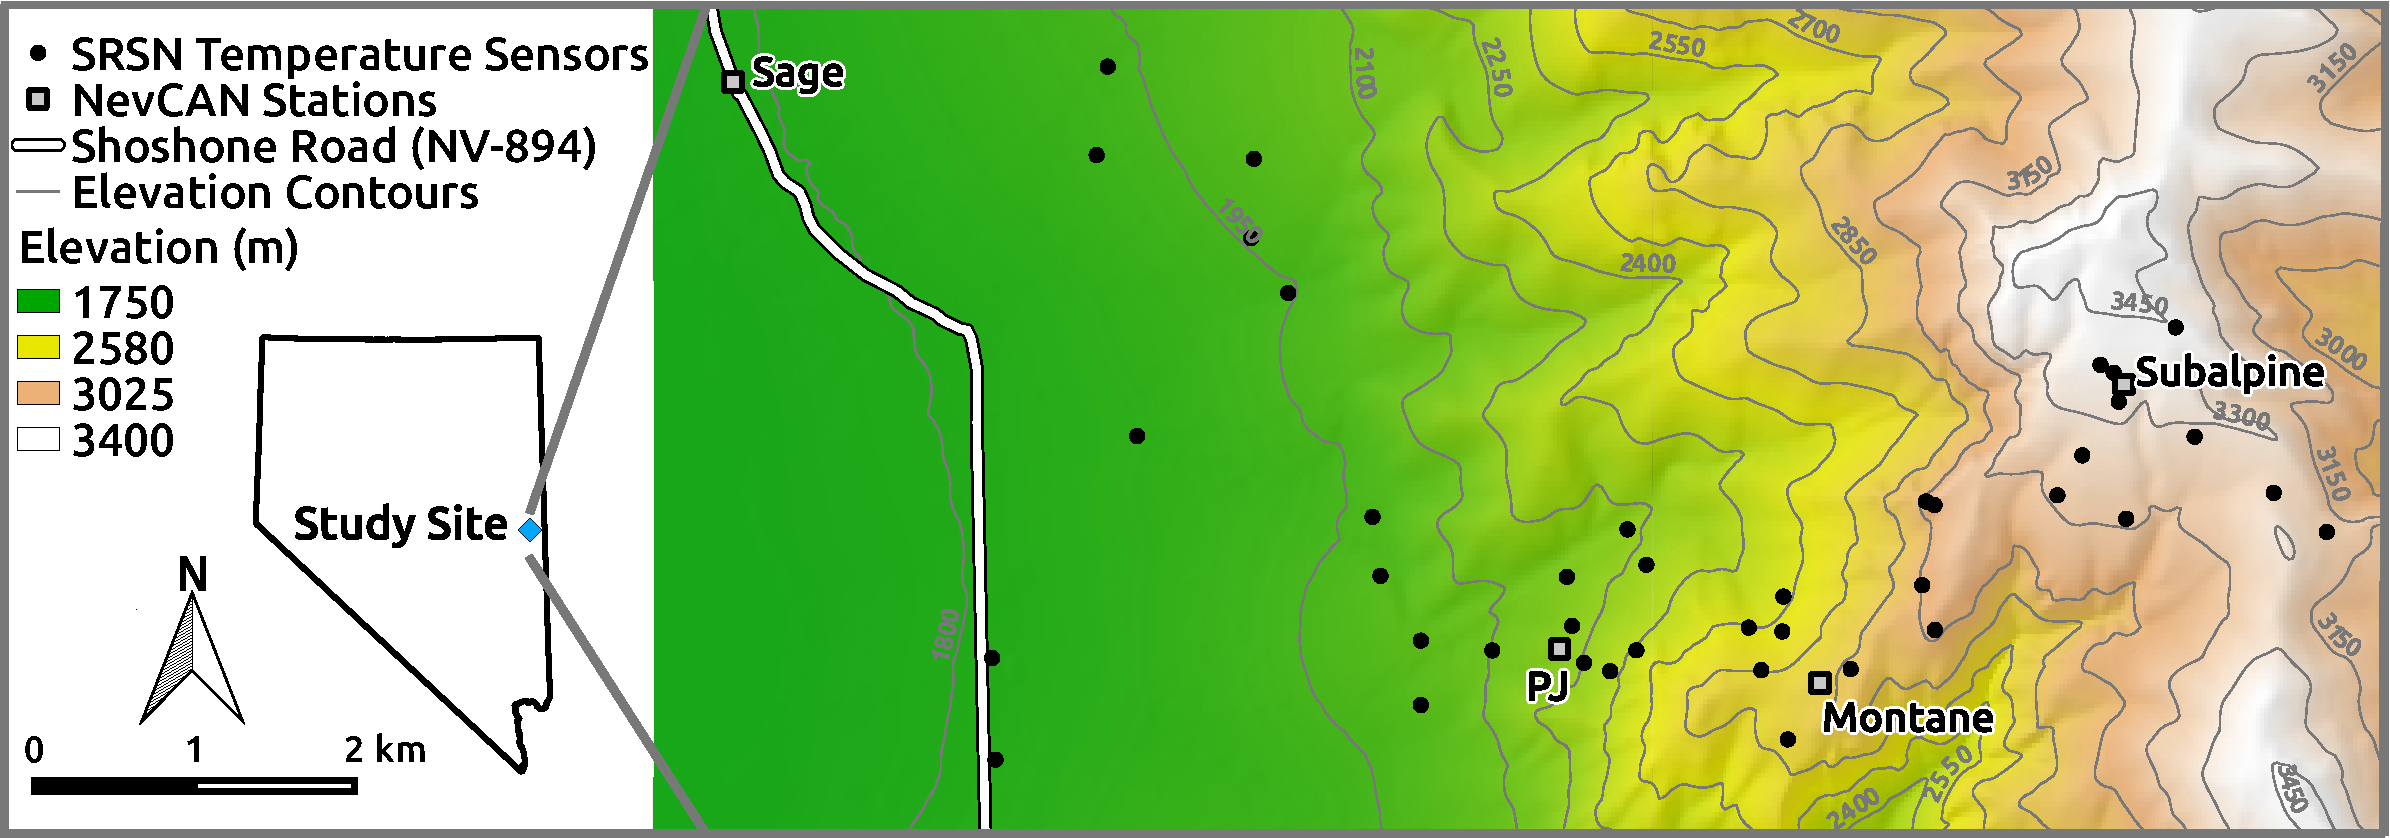
\includegraphics[width=39pc]{figure01_study-site.pdf}}

  \caption{A map of the study site in the Snake Range, Nevada, USA.  The blue diamond
  indicates the location of this study within the state of Nevada.  The
  Snake Range Sensor Network (SRSN) locations are shown as black points on the map
  and the NevCAN weather stations are indicated by the gray squares and
  labeled by name.  Colored shading indicates elevation, 
  the gray lines are elevation contours spaced at 150 m, and the white line represents
  Shoshone Road (NV-894).}\label{fig:1}

\end{figure}


%% Figure 2, EOF maps
\begin{figure}[ht]

 \centerline{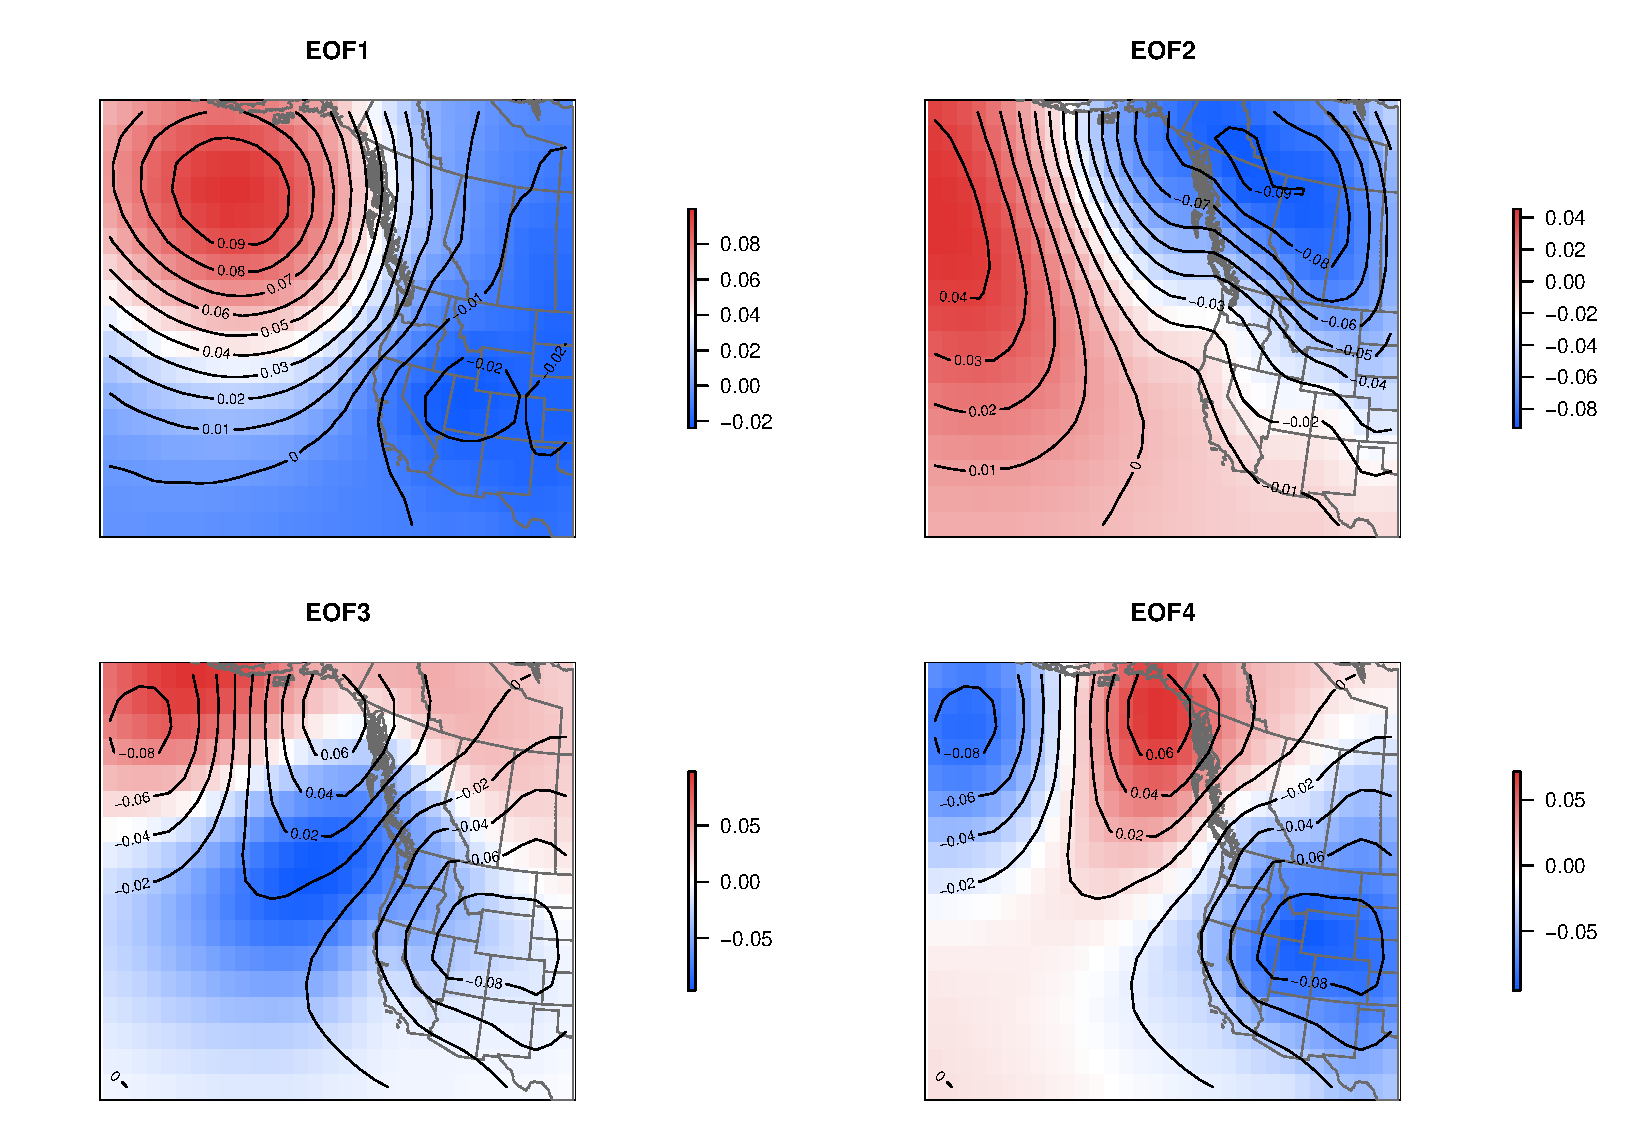
\includegraphics[width=39pc]{figure02_EOFs.pdf}}

  \caption{The first 4 of 544 empirical orthogonal functions (EOFs) identified by an empirical orthogonal function
  analysis of daily mean sea level pressure (SLP) anomalies.  Physical interpretation of these
  EOFs can be found in text.  The variation of these spatial patterns through time as Principle 
  Components (PCs) can be observed in Figure \ref{fig:3}, where the numeric label of each PC corresponds
  to the numeric label of these EOFs.}\label{fig:2}

\end{figure}


%% Figure 3, PC Time series
\begin{figure}[ht]

 \centerline{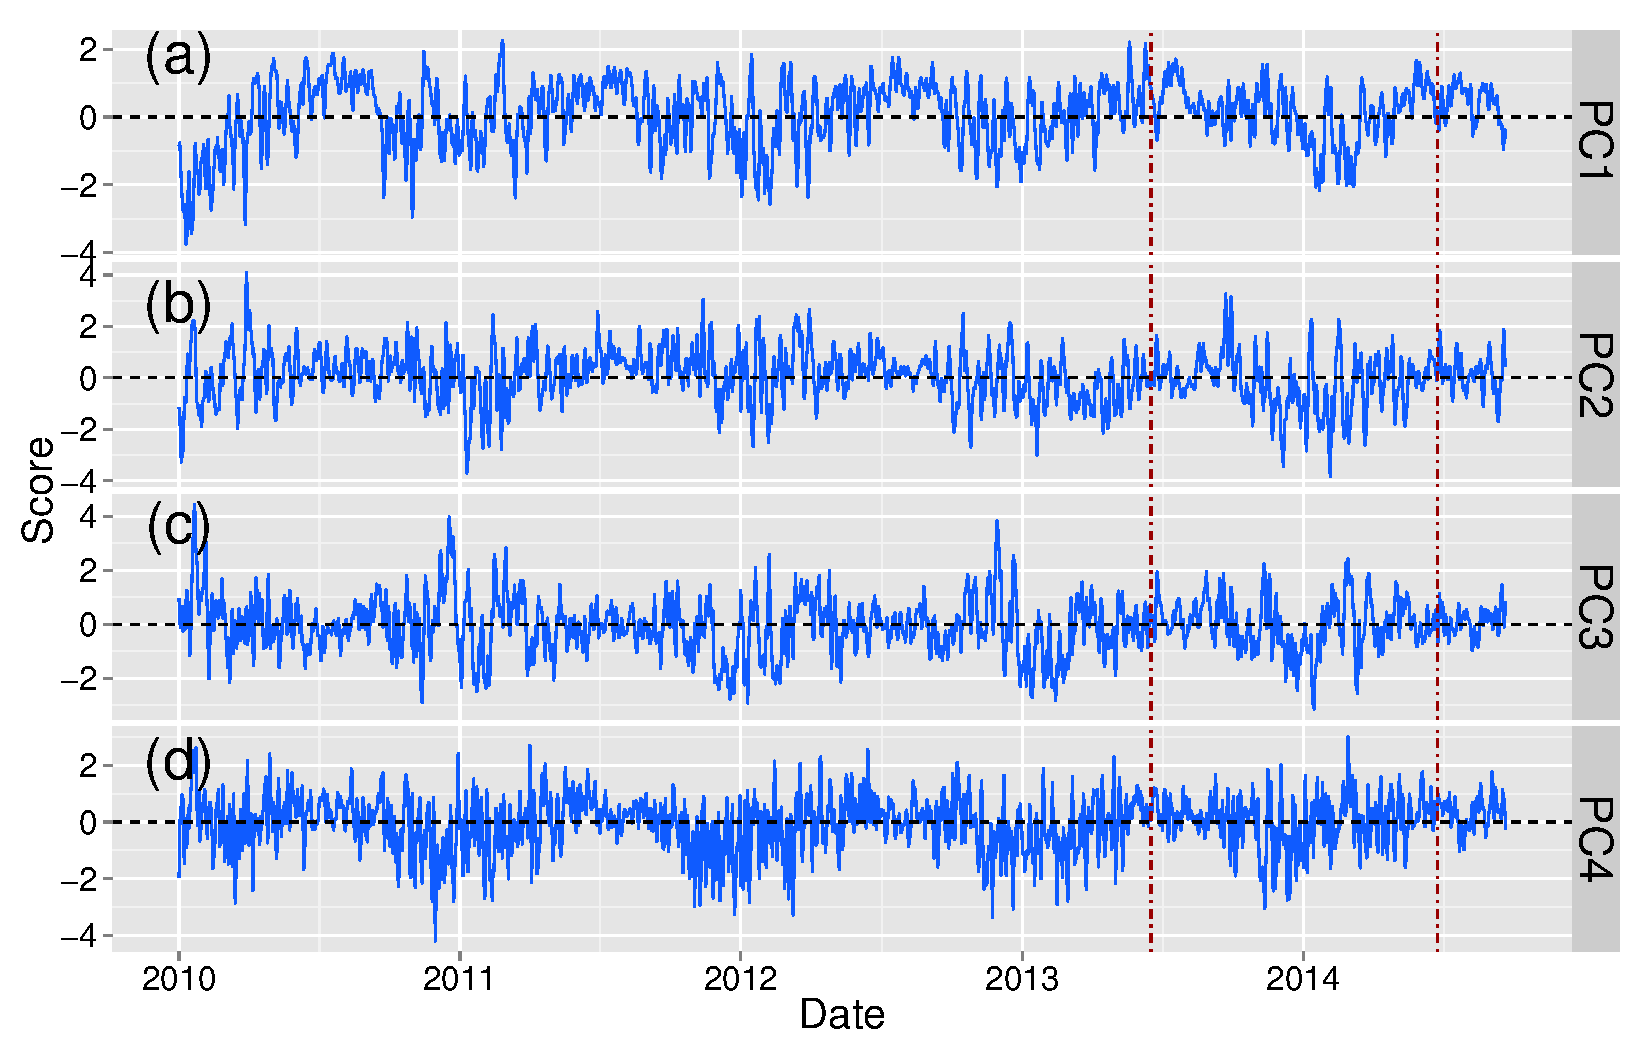
\includegraphics[width=39pc]{figure03_PCs.pdf}}

  \caption{The first 4 of 544 principle components (PCs) identified and described in text.  A temporal subset spanning 1 January 2009 to the final day of the analysis period, 24 September 2014, is displayed for clarity. Also note the differing y-axes, as the PC scores are relative. The vertical red lines indicate the portion of the time series that coincides with the Snake Range Sensor Network analysis period.}\label{fig:3}

\end{figure}


%% Figure 4, sensor data and Reanalysis air temp
\begin{figure}[ht]

\centerline{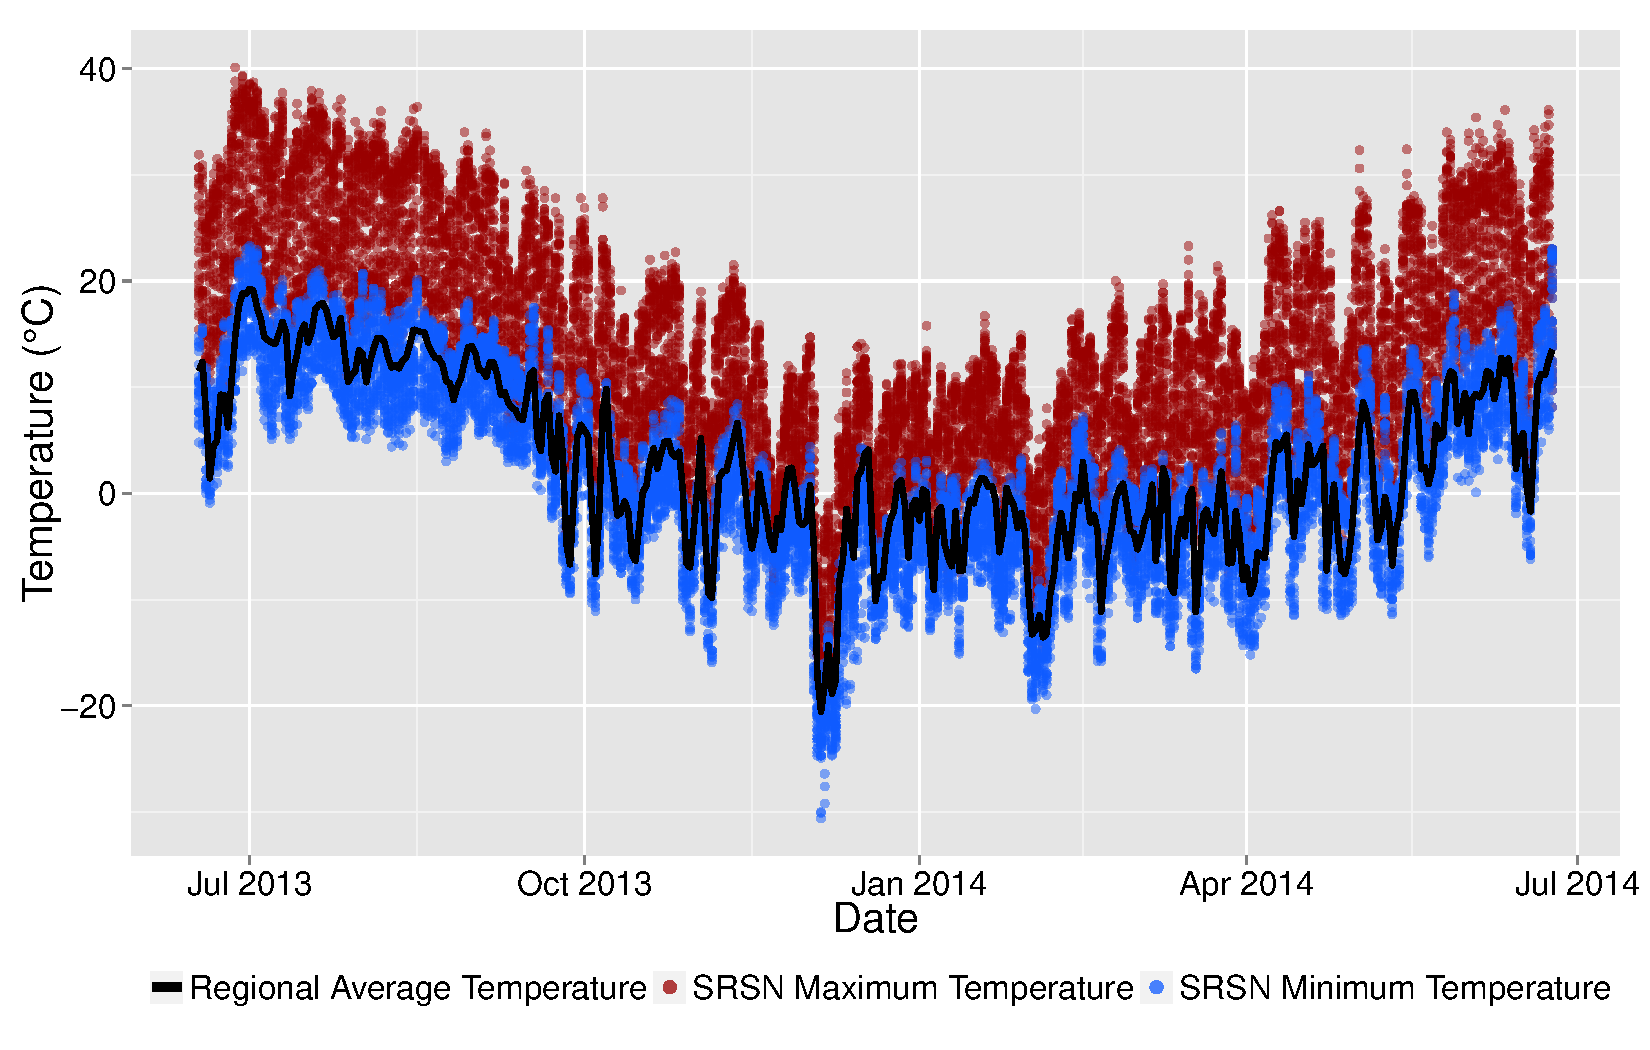
\includegraphics[width=39pc]{figure04_raw-t-data.pdf}}

 \caption{A time series showing all SRSN maximum and minimum daily temperature data collected during the study period (17 June 2013 to 24 June 2014) as red and blue symbols, respectively, and the NCEP Reanalysis 1 daily average air temperature at the 700 hPa level drawn as a black line. All of the SRSN $T_{max}$ and $T_{min}$ data are plotted for each day, thus up to 80 dots are present on each day. Note that data points are drawn as semitransparent, thus dark values indicate darker shades of red and blue indicate numerous observations. We intentionally chose color the data by sites for simplicity of viewing.}\label{fig:4}

\end{figure}


%% Figure 5, min temperature residuals vs tci by month
\begin{figure}[ht]

\centerline{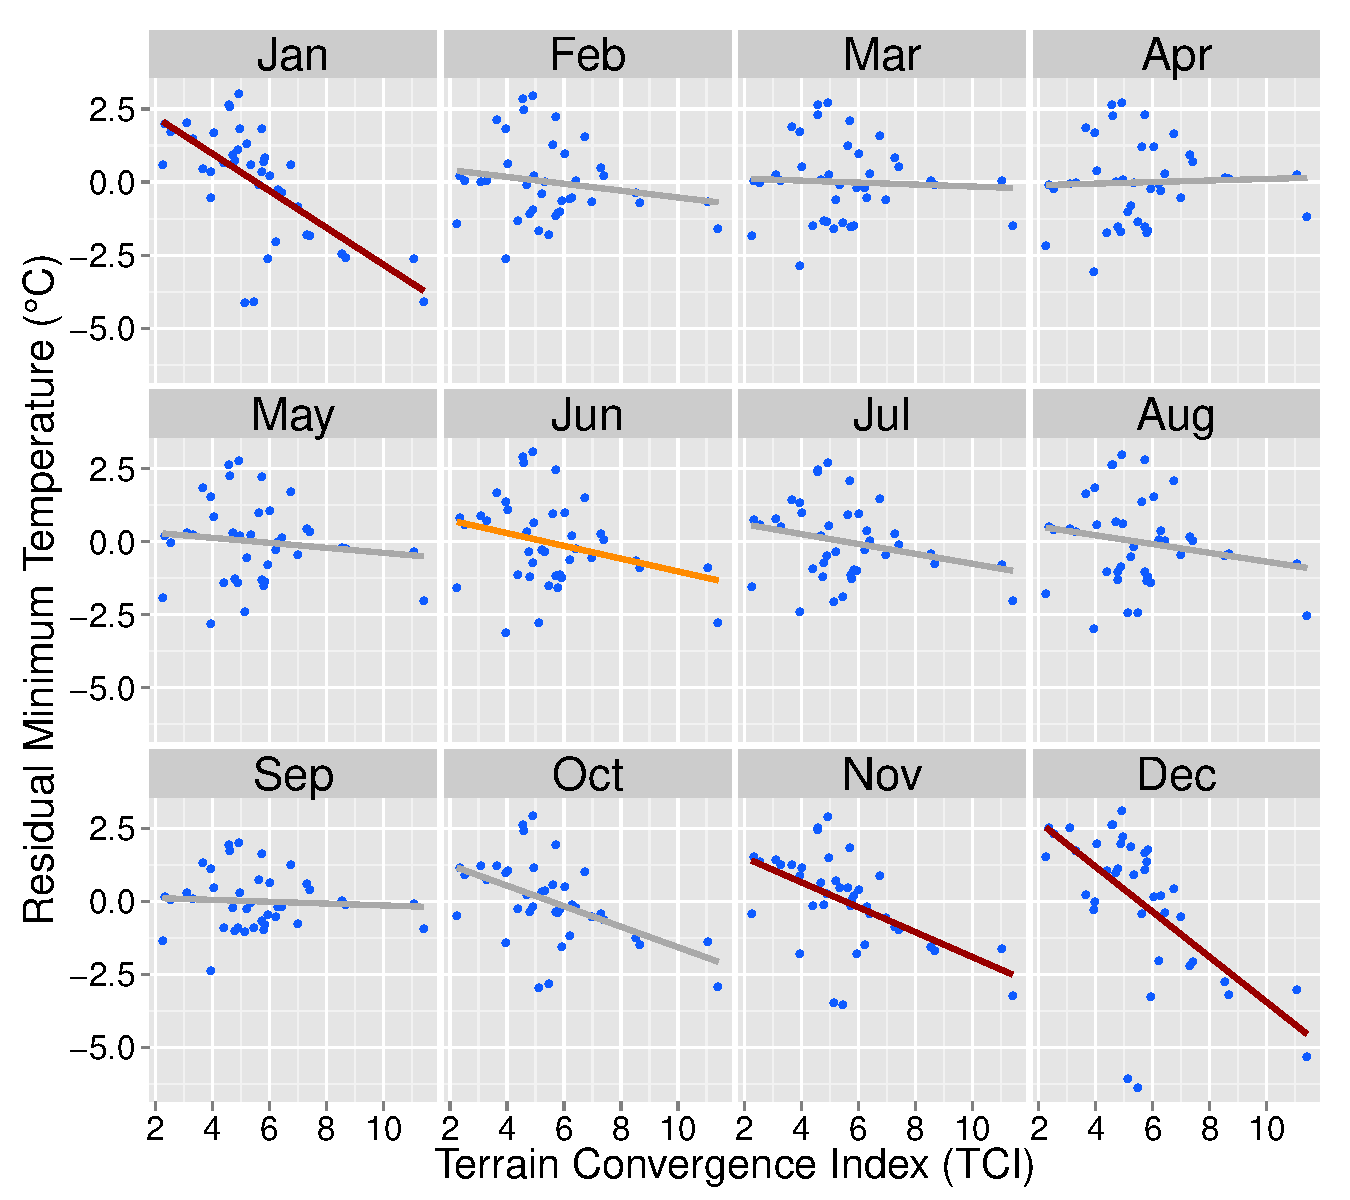
\includegraphics[width=39pc]{figure05_tci-elev-resid.pdf}}

 \caption{Modeling of minimum daily temperature averaged over the course of a month between 17 June 2013 and 24 June 2014 expressed as a function of terrain convergence index (TCI). Temperature is expressed as the residual of a mixed-effect model fit to the entirety of the SRSN data predicted solely by elevation with random intercepts by month. Residuals were then averaged for each site per month, and plotted against the TCI value at each sensor. The lines are fit by least squares regression. Lines are colored by the p-value associated with these least square regressions, where red indicates significance at the 0.05 level (p $<$ 0.05), orange indicates significance at the 0.10 level (p $<$ 0.10), and gray indicates no significance at the 0.10 level (p $>$ 0.10).}\label{fig:5}

\end{figure}

%% Figure 6, maximum temperature residuals vs slope by month
\begin{figure}[ht]

\centerline{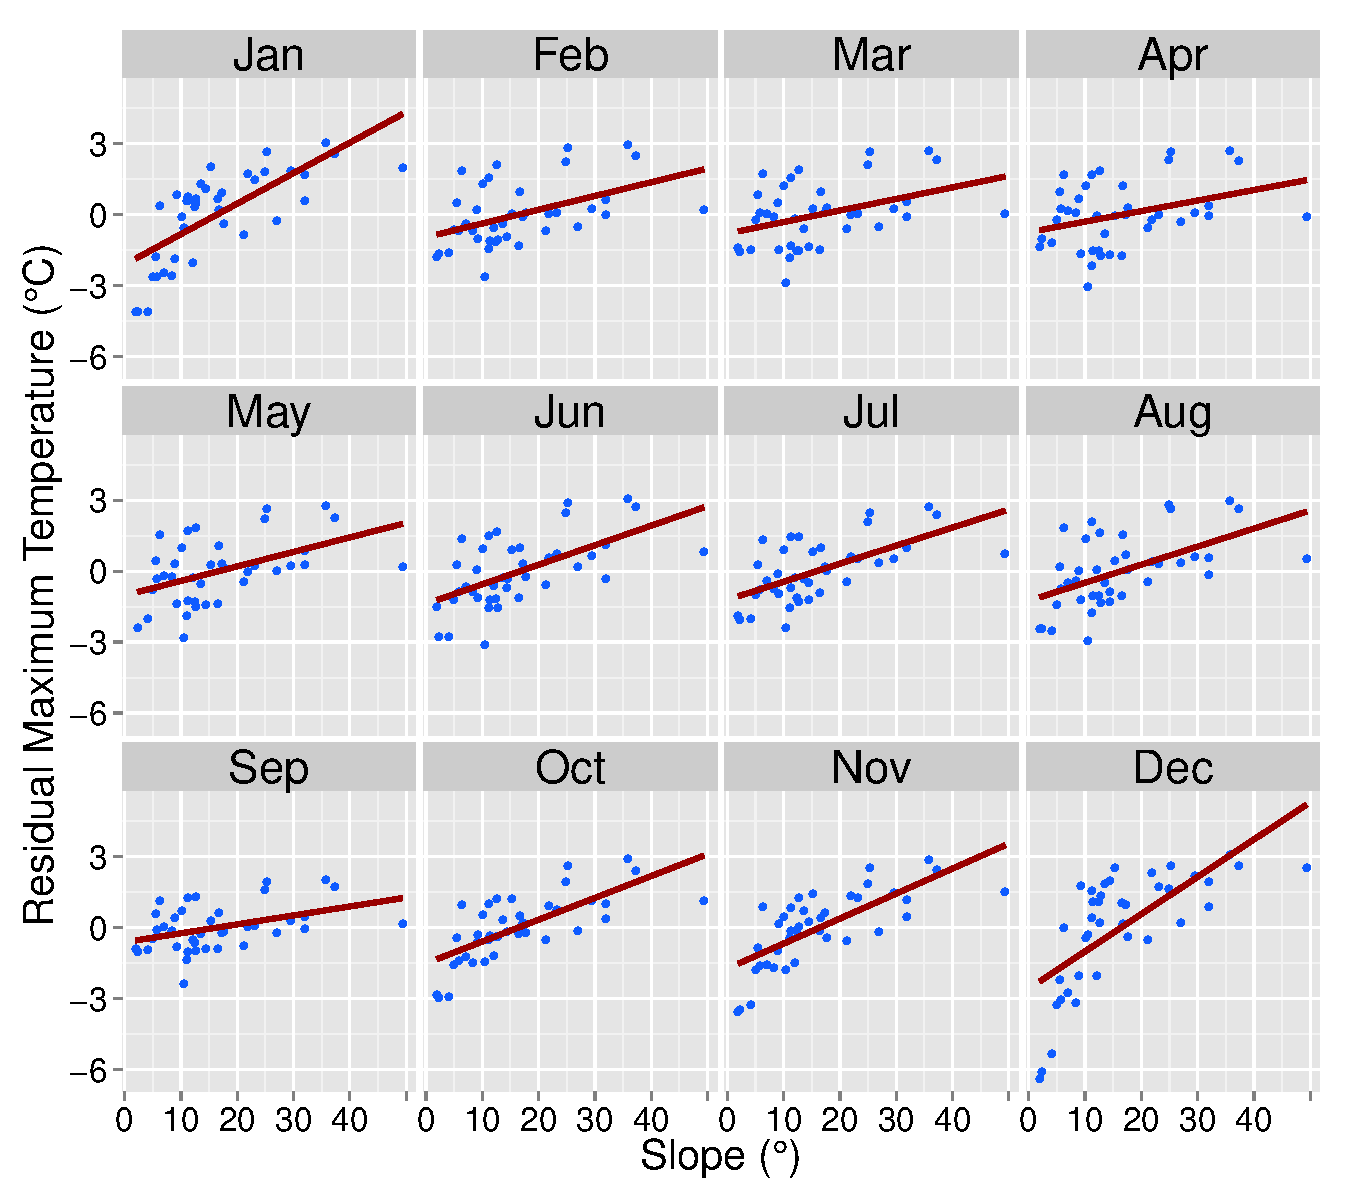
\includegraphics[width=39pc]{figure06_slope-elev-resid.pdf}}

\caption{Modeling of maximum daily temperature averaged over the course of a month between 17 June 2013 and 24 June 2014 expressed as a function of terrain slope ($\degree$). Temperature is expressed as the residual of a mixed-effect model fit to the entirety of the SRSN data predicted by elevation with random intercepts by month. Residuals were then averaged for each site per month and plotted against the terrain slope at each sensor. The lines are fit by least squares regression. All months were statistically significant at the 0.05 level (p < 0.05).\label{fig:6}}

\end{figure}


%% Figure 7, validation of tmn model
\begin{figure}[ht]

\centerline{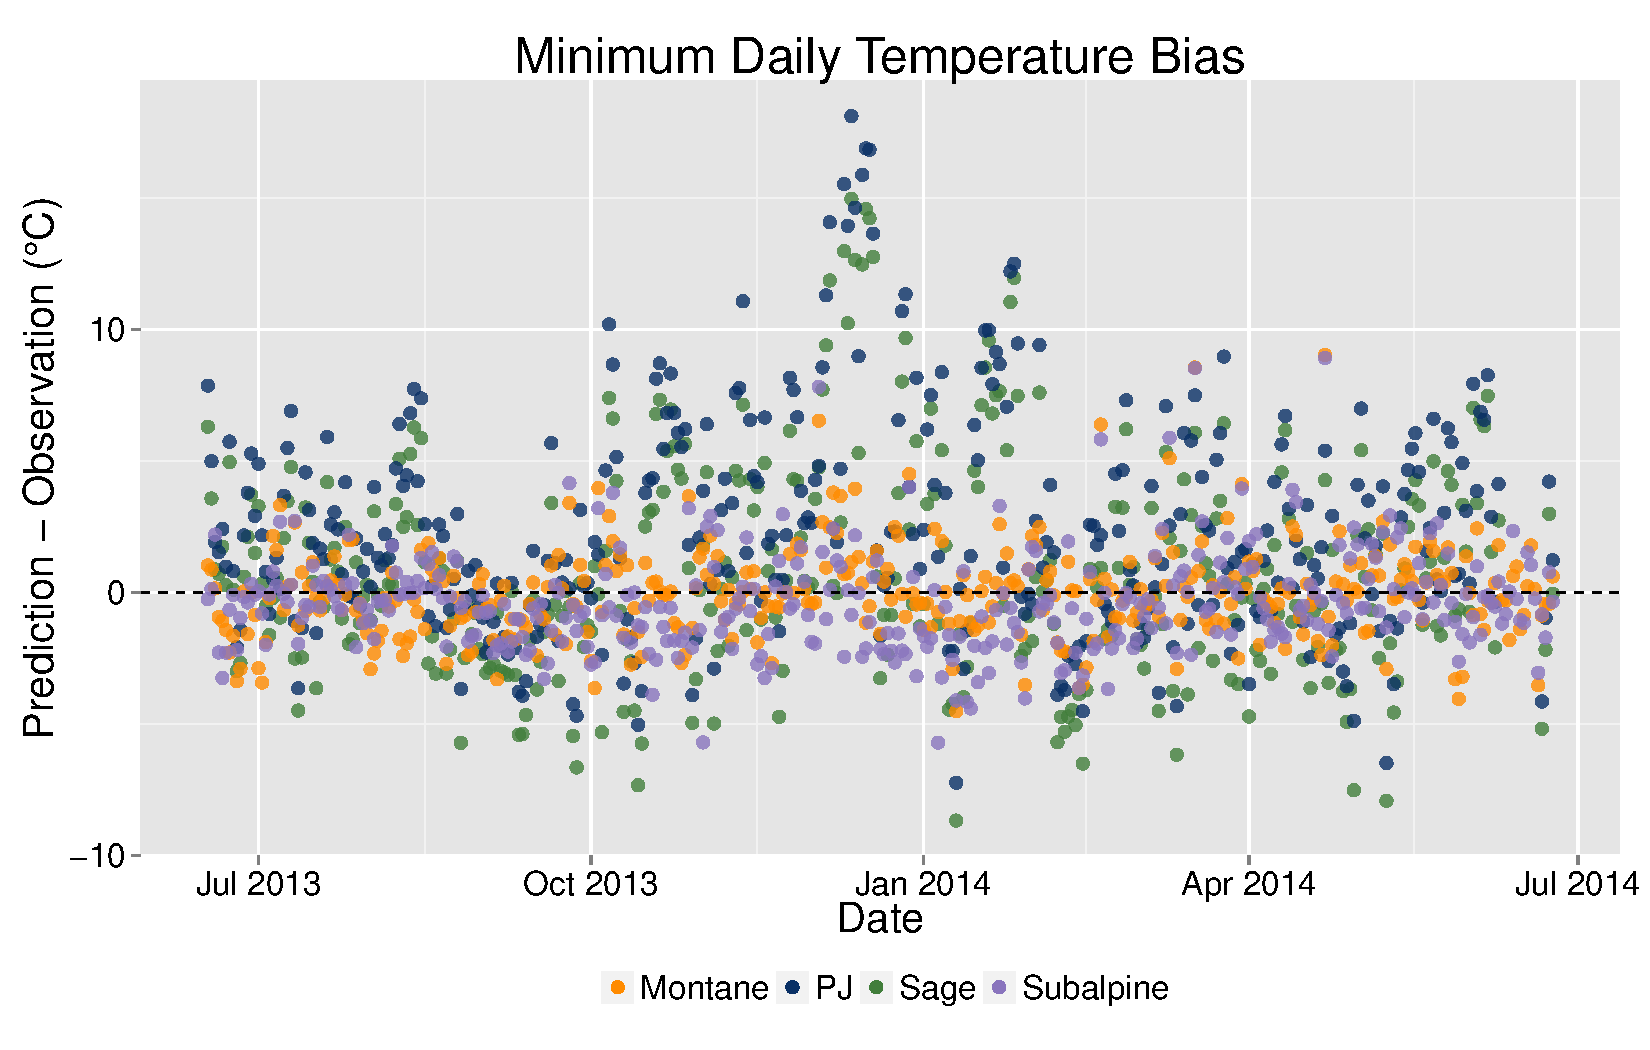
\includegraphics[width=39pc]{figure07_tmn-validation.pdf}}

\caption{Difference between daily minimum temperature ($\degree$C) as predicted by the hierarchical mixed-effects model described in text and observed daily minimum temperature at 4 NevCAN stations over time. The Montane site is visualized as orange dots, the Pinyon-Juniper site (PJ) is dark blue, the Sagebrush (Sage) site is dark green, and the Subalpine site is purple. The black horizontal line represents a perfect prediction.\label{fig:7}}

\end{figure}


%% Figure 8, validation of tmx model
\begin{figure}[ht]

\centerline{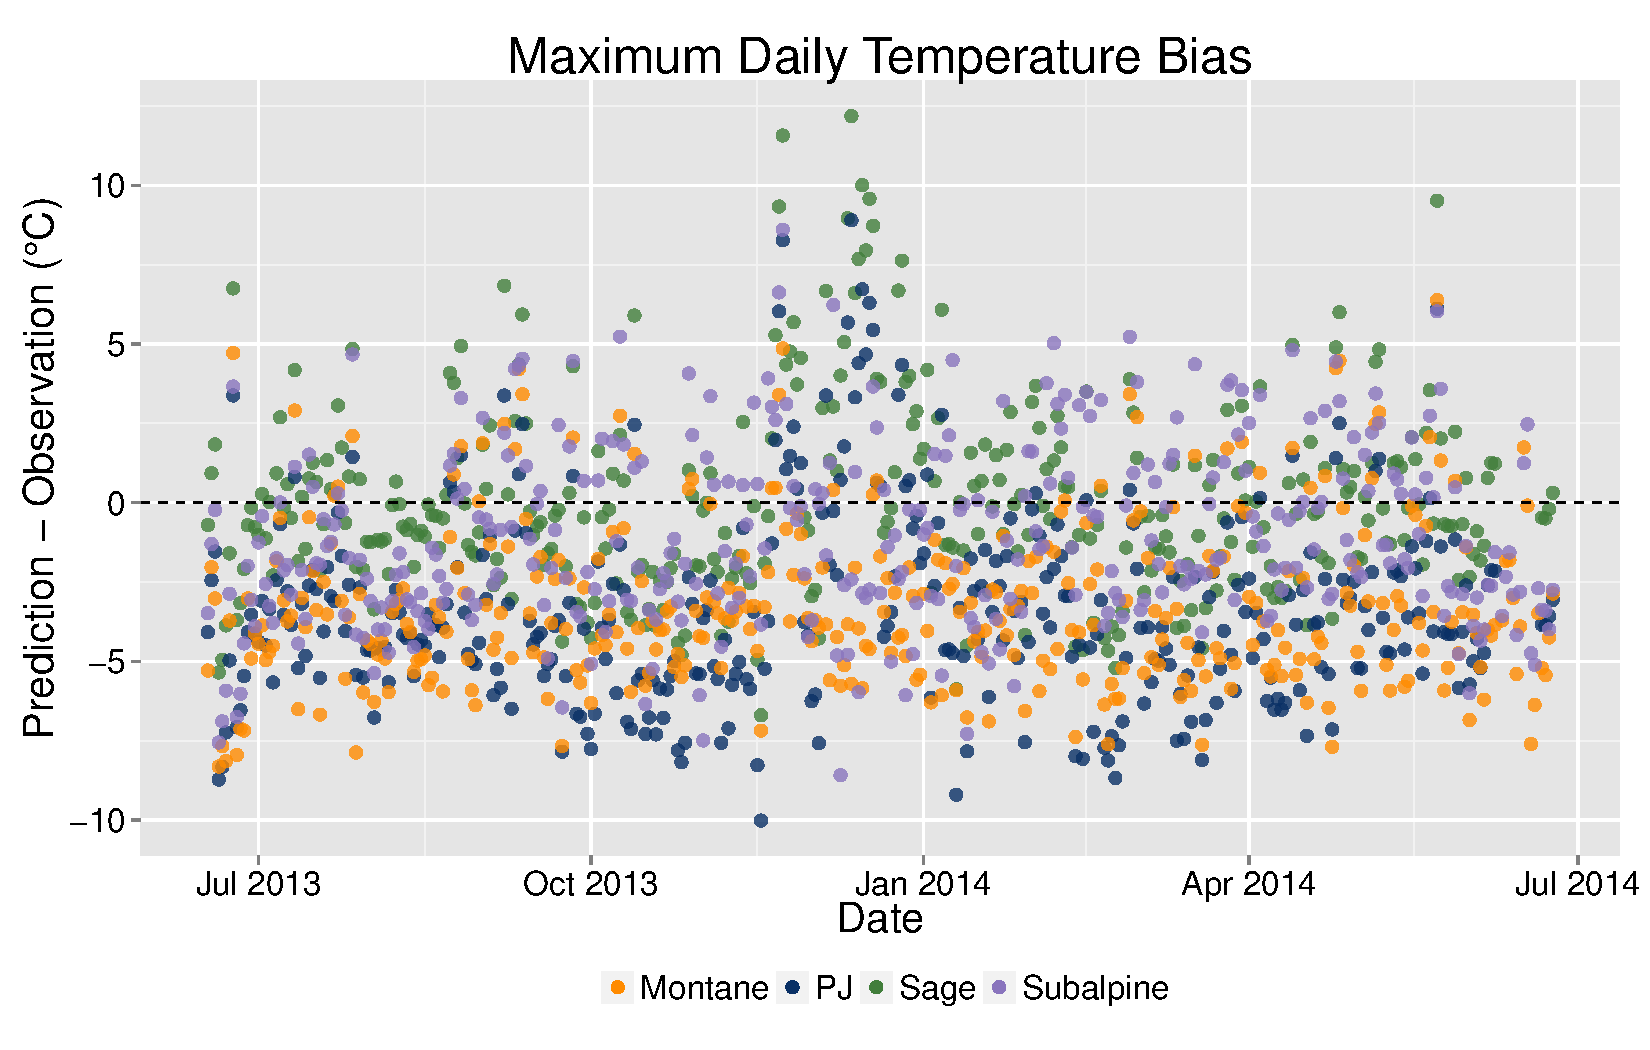
\includegraphics[width=39pc]{figure08_tmx-validation.pdf}}

\caption{Difference between daily maximum temperature ($\degree$C) as predicted by the hierarchical mixed-effects model described in text and observed daily maximum temperature at 4 NevCAN stations over time. The Montane site is visualized as orange dots, the Pinyon-Juniper site (PJ) is dark blue, the Sagebrush (Sage) site is dark green, and the Subalpine site is purple. The black horizontal line represents a perfect prediction.\label{fig:8}}

\end{figure}

%% Figure 9, Temperature maps
\begin{figure}[ht]

\centerline{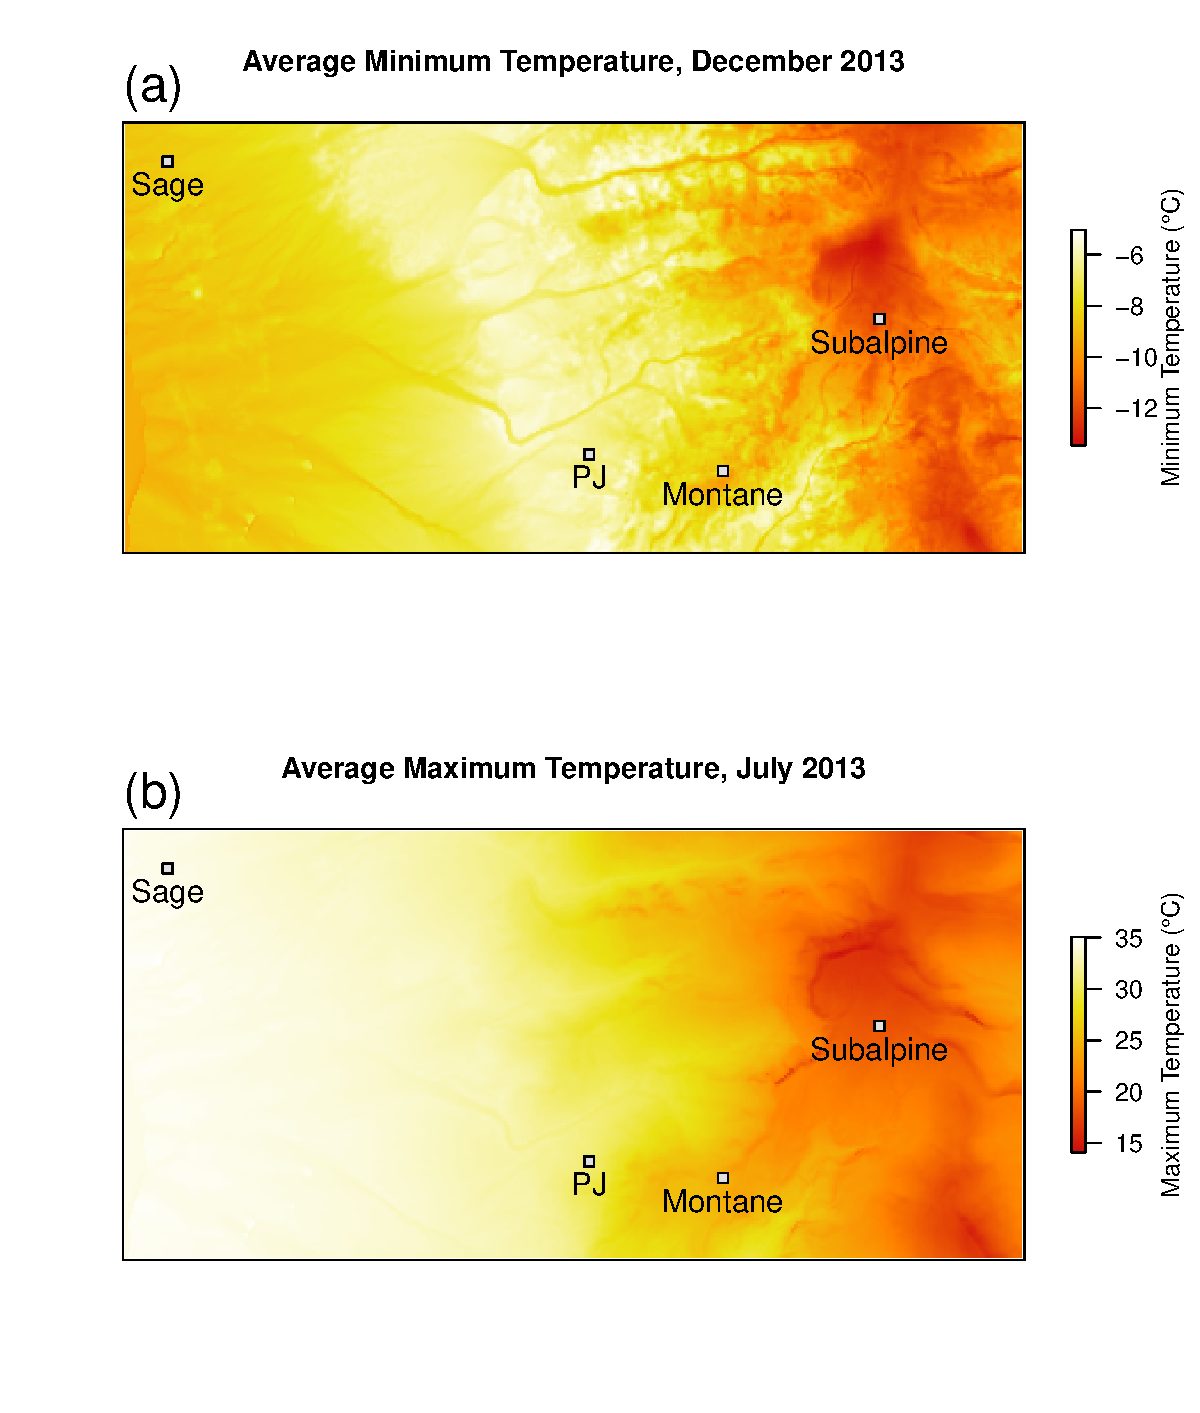
\includegraphics[width=39pc]{figure09_temperature-maps.pdf}}

\caption{Two maps of temperature as predicted by the models described in text. Gray squares indicate NevCAN stations, which were used as validation sites in this work. Scale and orientation are the same as Figure 1. Note that (a) and (b) have different legends and are for different time periods. (a) A map of average minimum temperature throughout the study site, calculated by taking the mean of daily minimum temperature for the month of December 2013. (b) A map of average maximum temperature, calculated by taking the mean of daily maximum temperature predictions for the month of July 2013.\label{fig:9}}

\end{figure}


%% Figure 10, tmn lapse rates
\begin{figure}[ht]

\centerline{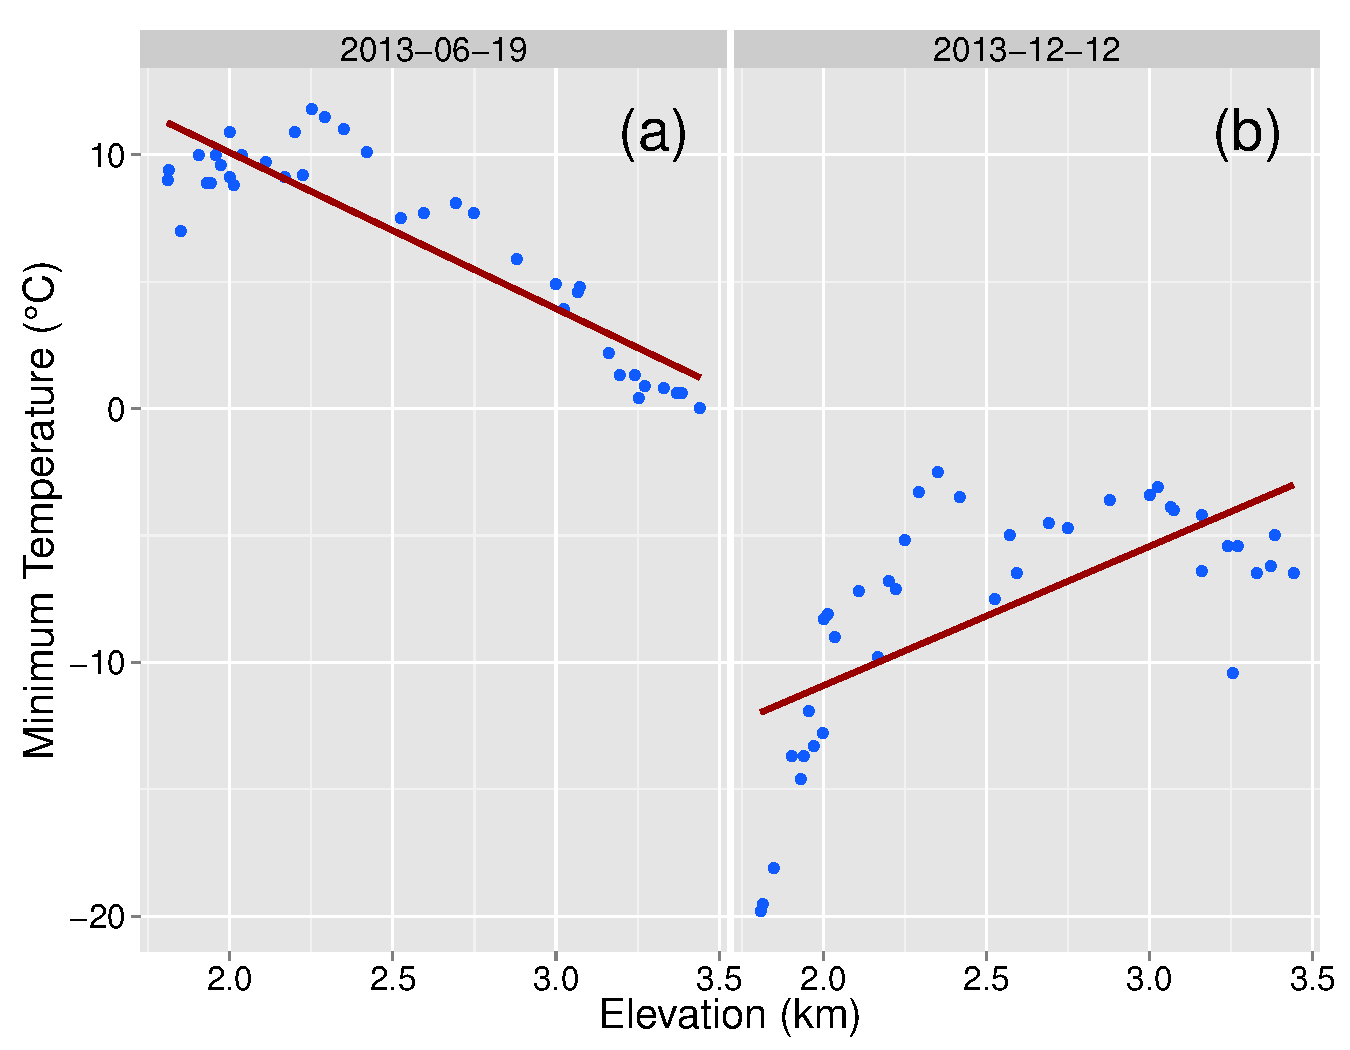
\includegraphics[width=39pc]{figure10_tmn-lapse.pdf}}

\caption{Minimum temperature across the 40 sites of the SRSN on two separate days plotted against site elevation. The panel on the left is from 2013 June 19, and it displays the more typical pattern of $T_{min}$ for the area. Minimum temperature at the lower elevation sites is relatively constant, as cold air drainage occurs on a nearly nightly basis at the site. The right pane shows minimum temperature recorded by the SRSN plotted against elevation. This particular day shows a deep inversion present at the study site, where temperature increases with elevation rather than decreases. The red lines represent a least squares linear regression model that has been fit to the data, which is often thought of as the lapse rate.}
\label{fig:10}
\end{figure}


\begin{figure}[ht]

\centerline{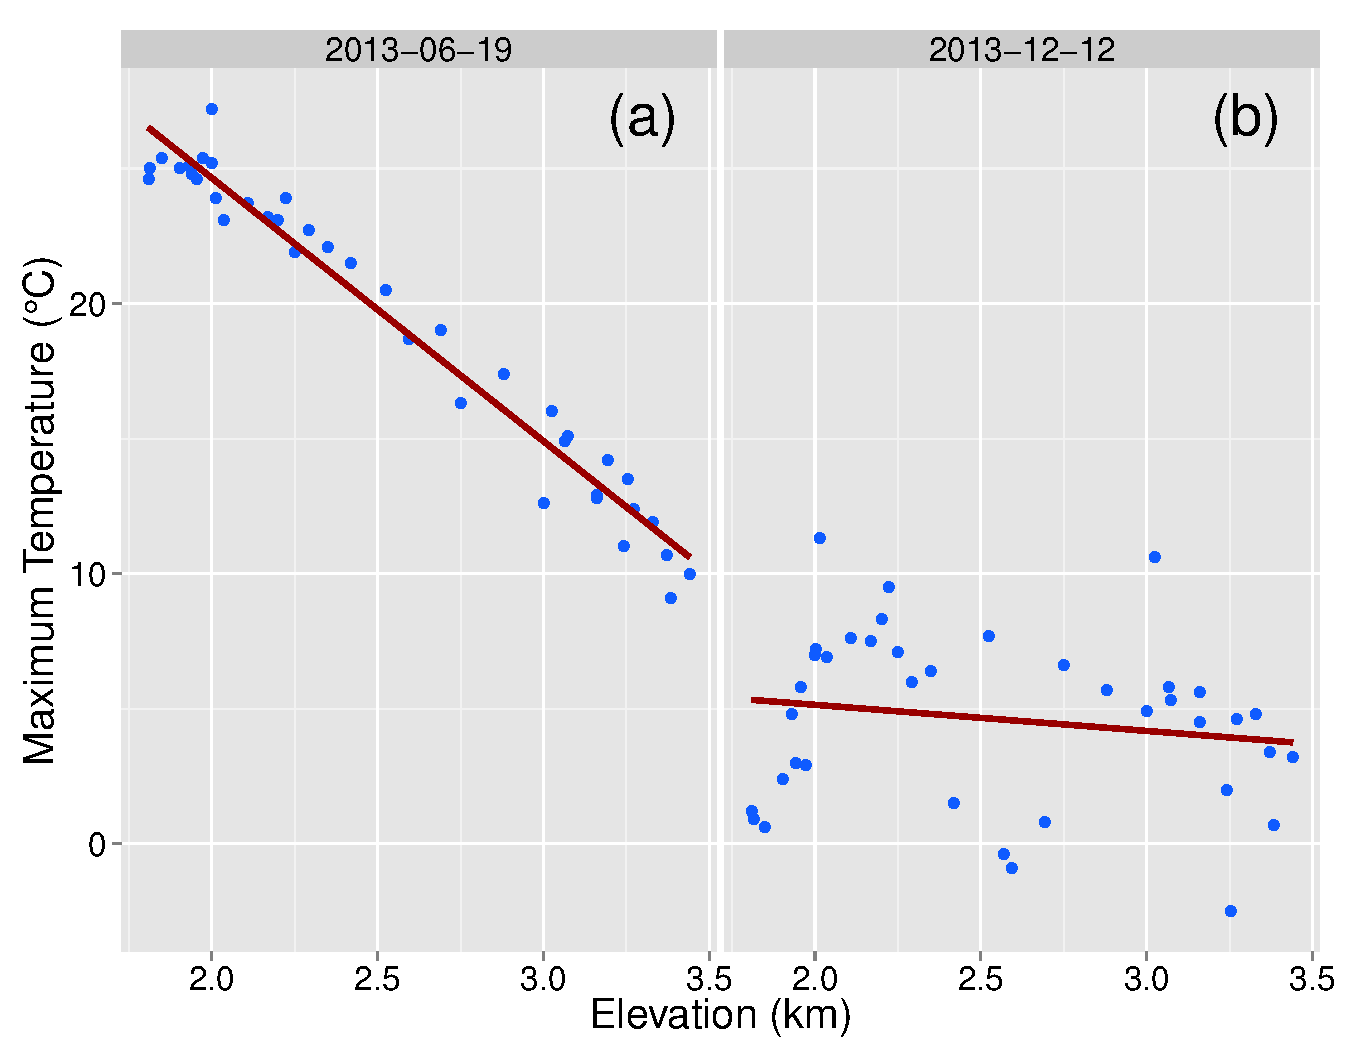
\includegraphics[width=39pc]{figure11_tmx-lapse.pdf}}

\caption{Maximum temperature across the 40 sites of the SRSN on two separate days plotted against the elevation of each site, where red lines represent a least squares linear regression line fitted to the data, which is often thought of as the atmospheric lapse rate. (a) Maximum daily temperature from 2013 June 19. this displays a typical maximum temperature observation at the site, where maximum temperature decreases linearly with decreasing elevation. (b) Maximum daily temperature from 2013 December 12, which shows a persistent inversion occurring at the site. As you increase elevation, there is a very slight decrease in maximum temperature for that day.}
\label{fig:11}
\end{figure}


%%%%%%%%%%%%%%%%%%%%%%%%%%%%%%%%%%%%%%%%%%%%%%%%%%%%%%%%%%%%%%%%%%%%%
% END OF AMSPAPER.TEX
%%%%%%%%%%%%%%%%%%%%%%%%%%%%%%%%%%%%%%%%%%%%%%%%%%%%%%%%%%%%%%%%%%%%%
\end{document}


